\chapter{Appendix}
\section{Example code}

\section{Heatmaps of hypothesis tests}
\label{app:heatmaps}

This section contains heatmaps generated by applying hypthesis tests to samples of varying size sampled from a distribution of error metrics generated by the DeepAREstimator on the Electricity dataset. DeepAR was executed with three different values of the \textit{distr\_output} hyperparameter; NegativeBinomialOutput, StudentTOutput and PoissonOutput. The distributions generated by the different hyperparameter configurations are refered to as Negative Binomial, Student T and Poisson. See Section \ref{hypothesis_test_methodology} for more information about how the distributions were generated.

In the heatmaps, green means the test approves the samples being from the same distribution otherwise it is red.


\subsection{Kolmogorov Smirnov heatmaps of samples from a single distribution}

\begin{figure}[htb]
  \centering
  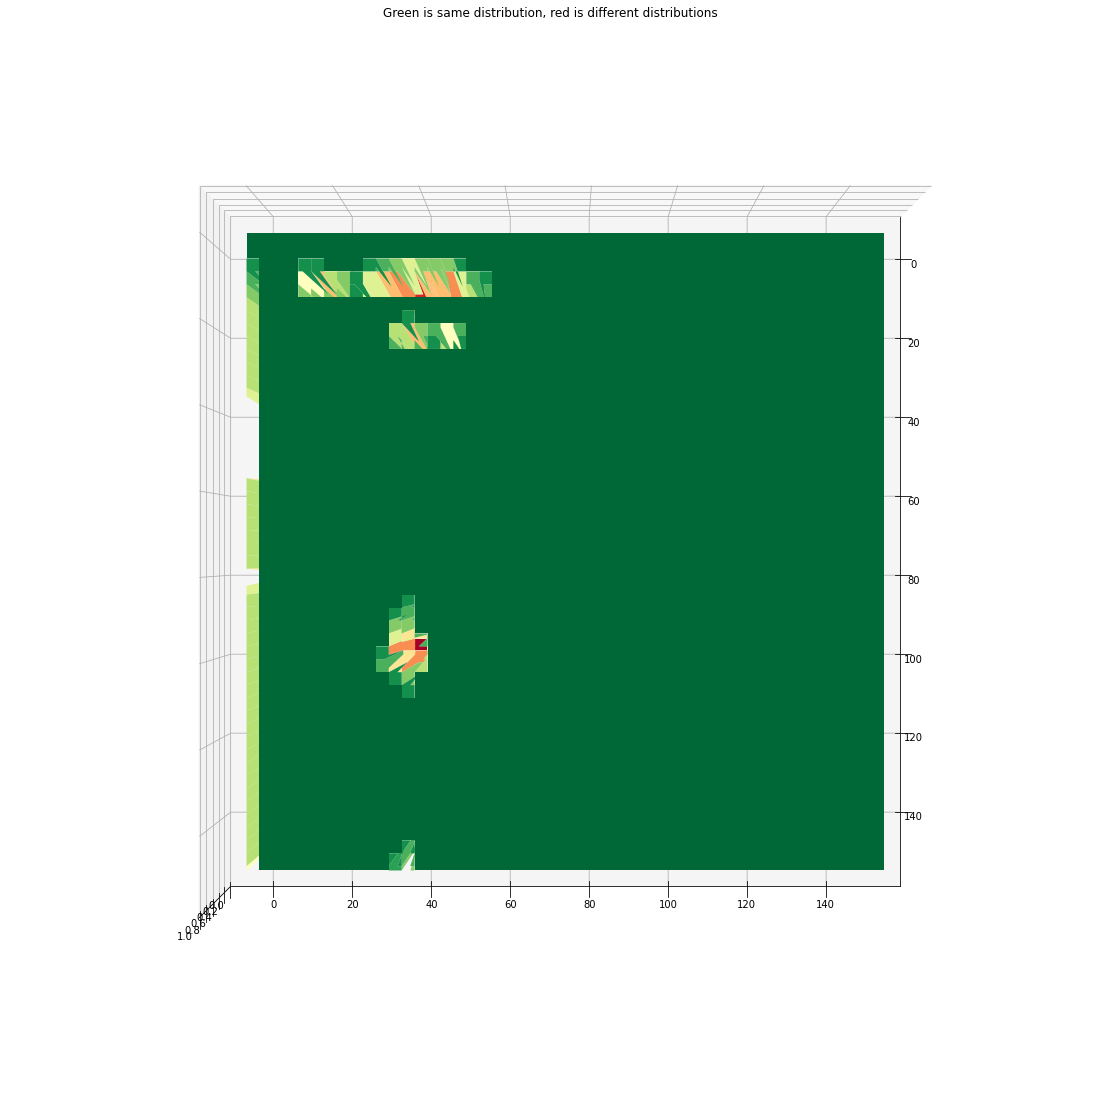
\includegraphics[width=\linewidth]{./img/hypothesis_test/appendix/ks_neg_bin.png}
  \caption{Negative Binomial}
\end{figure}
\clearpage
\begin{figure}[htb]
  \centering
  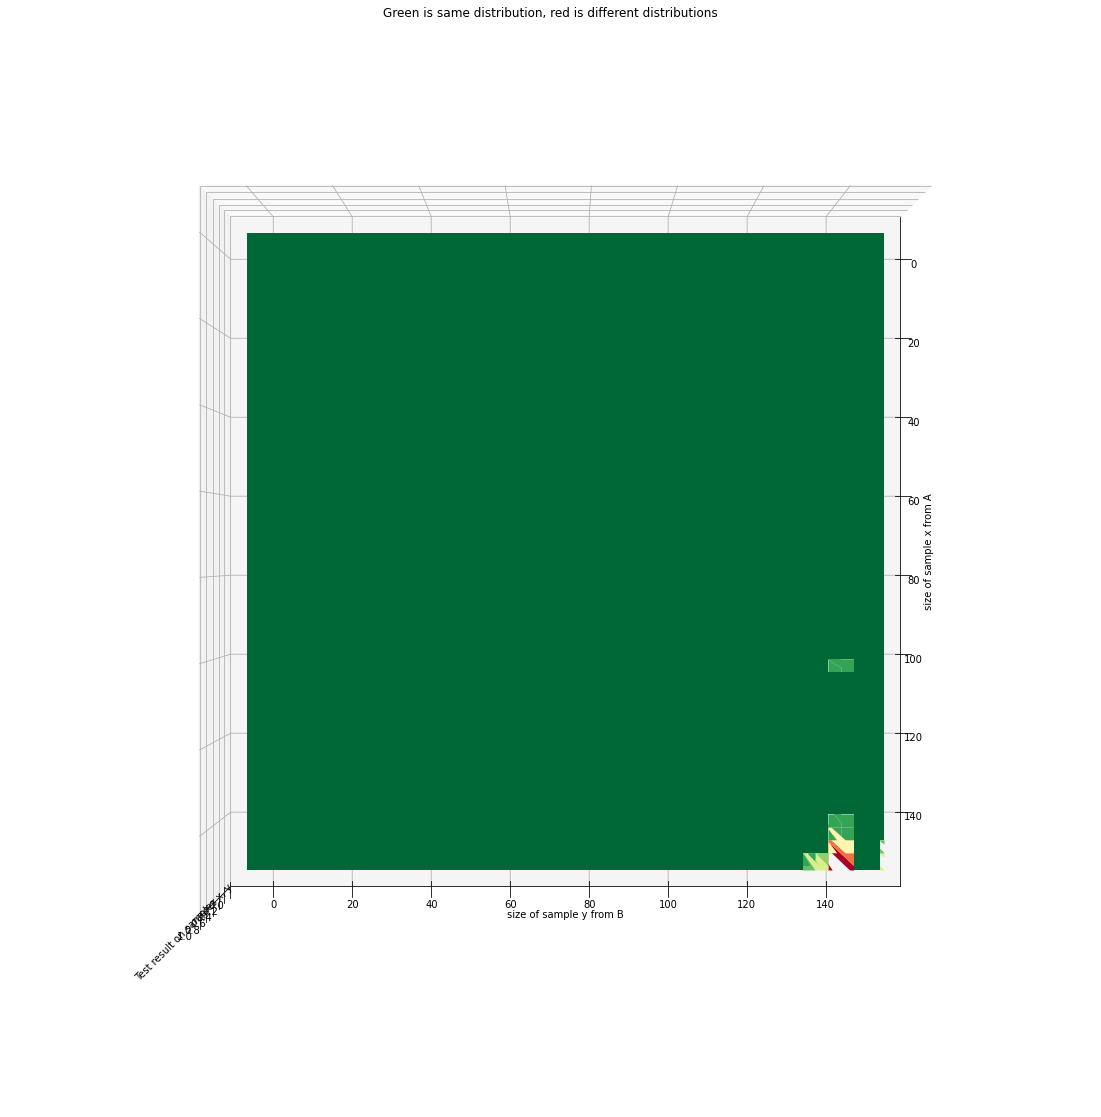
\includegraphics[width=\linewidth]{./img/hypothesis_test/appendix/ks_poisson.png}
  \caption{Poisson}
\end{figure}
\clearpage
\begin{figure}[htb]
  \centering
  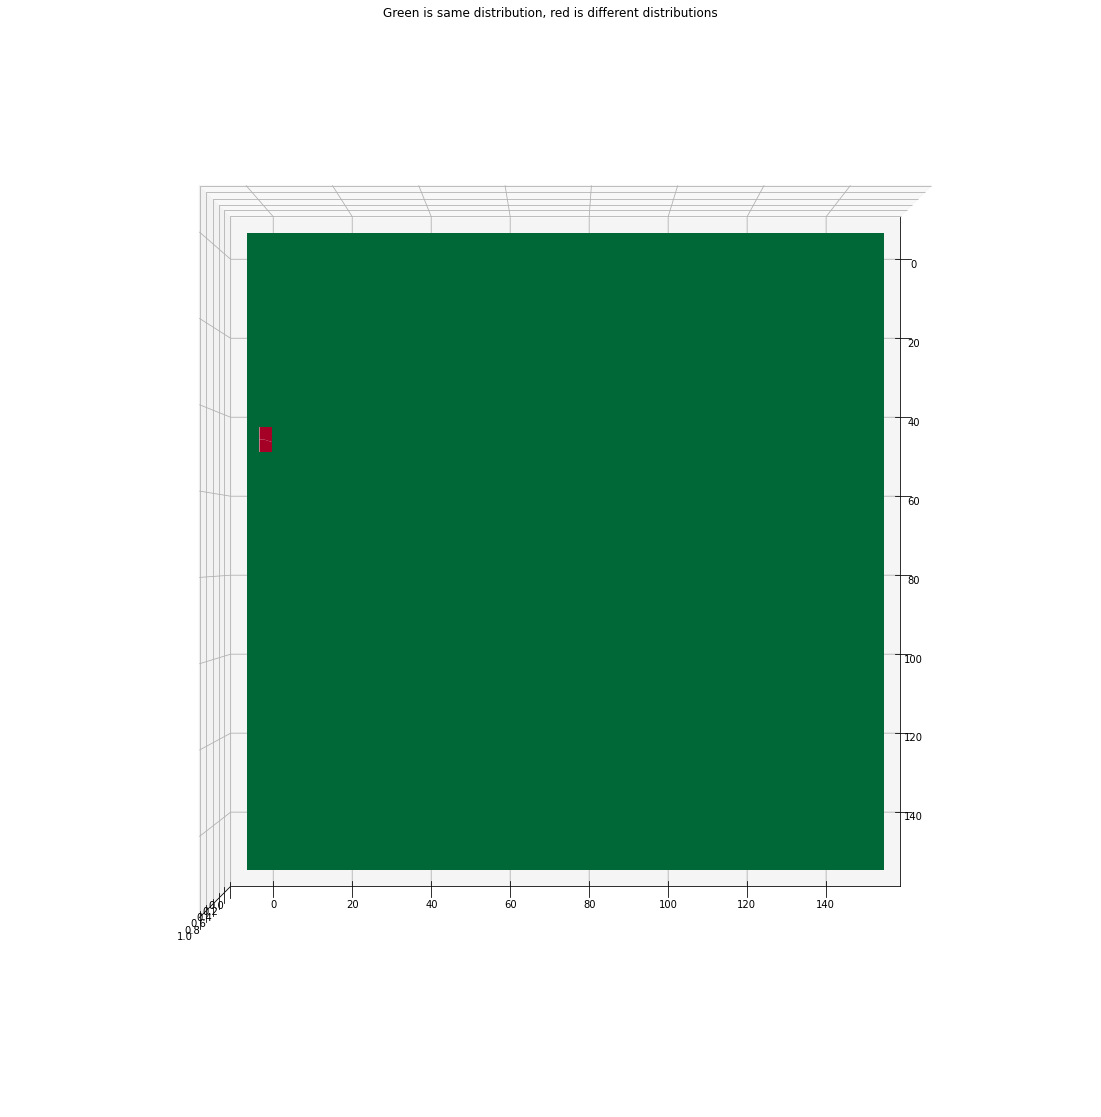
\includegraphics[width=\linewidth]{./img/hypothesis_test/appendix/ks_student_t.png}
  \caption{Student T}
\end{figure}
\clearpage

\subsection{Kolmogorov Smirnov heatmaps of samples from two independent and shuffled distributions}

\begin{figure}[htb]
  \centering
  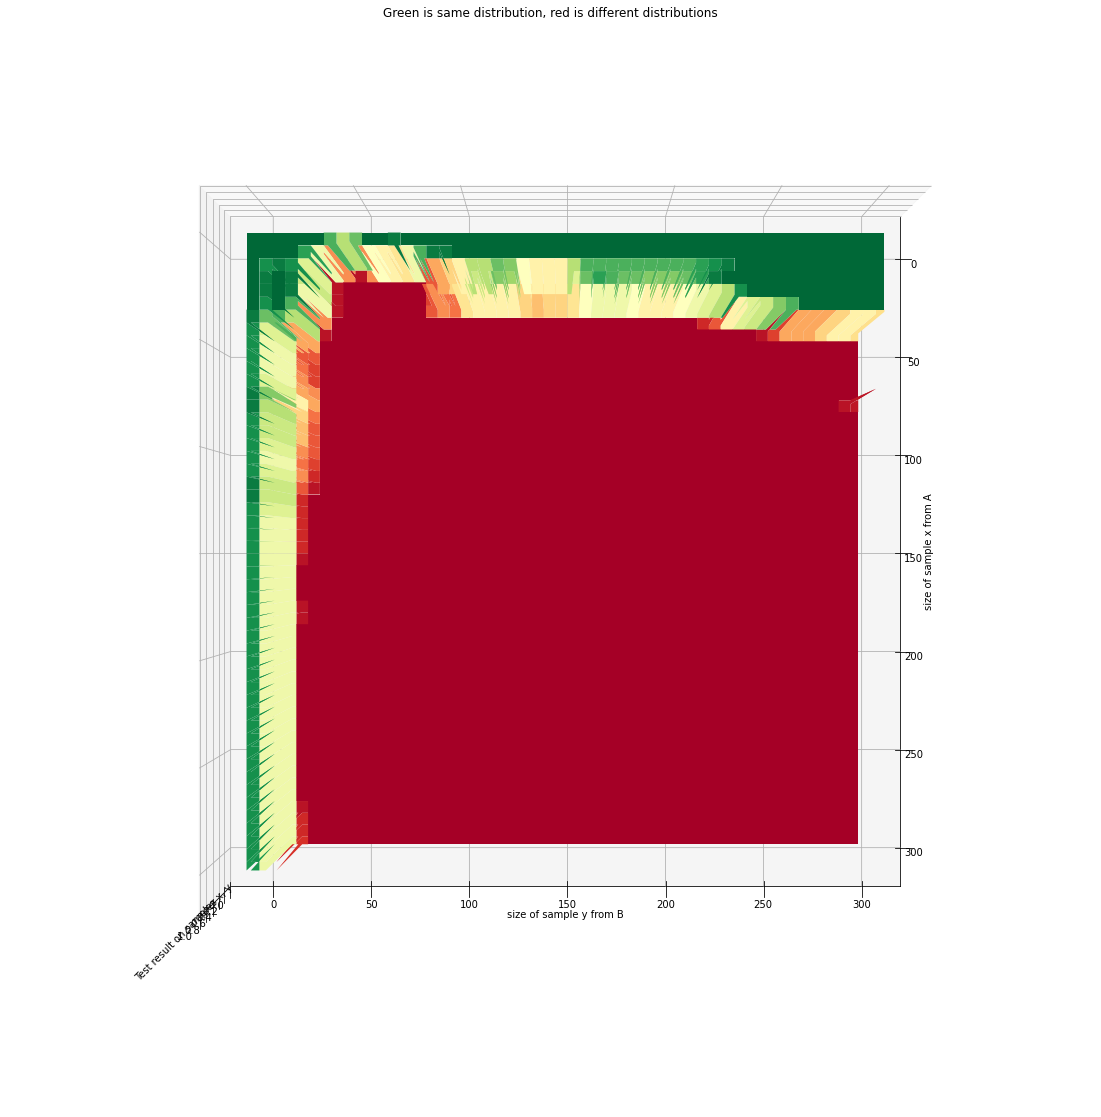
\includegraphics[width=\linewidth]{./img/hypothesis_test/appendix/ks_X_neg_bin_Y_student_t_shuffled.png}
  \caption{Negative Binomial on X axis and Student T on Y axis}
\end{figure}
\clearpage
\begin{figure}[htb]
  \centering
  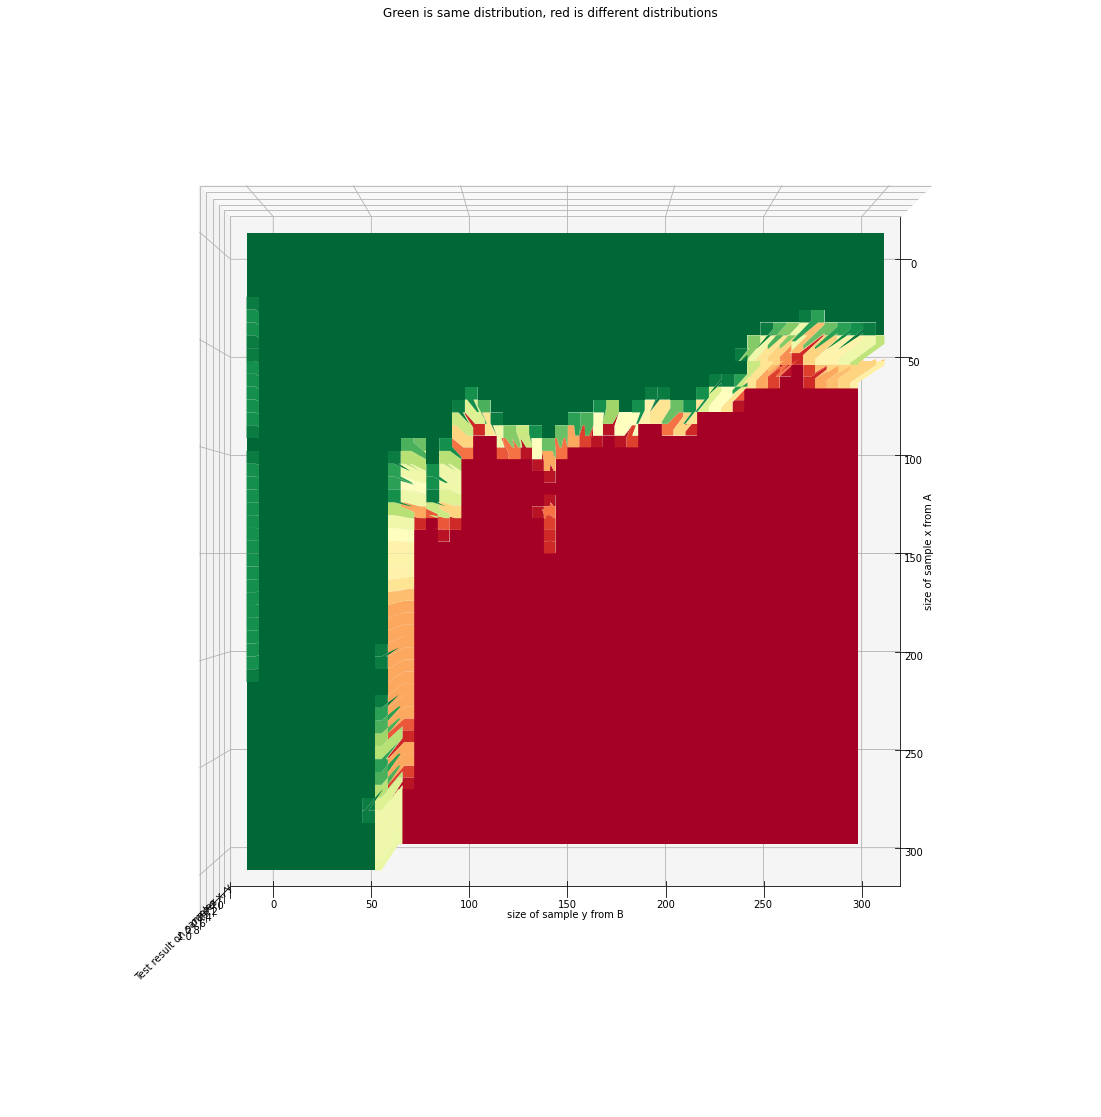
\includegraphics[width=\linewidth]{./img/hypothesis_test/appendix/ks_X_poisson_Y_neg_bin_shuffled.png}
  \caption{Poisson on X axis and Negative Binomial on Y axis}
\end{figure}
\clearpage
\begin{figure}[htb]
  \centering
  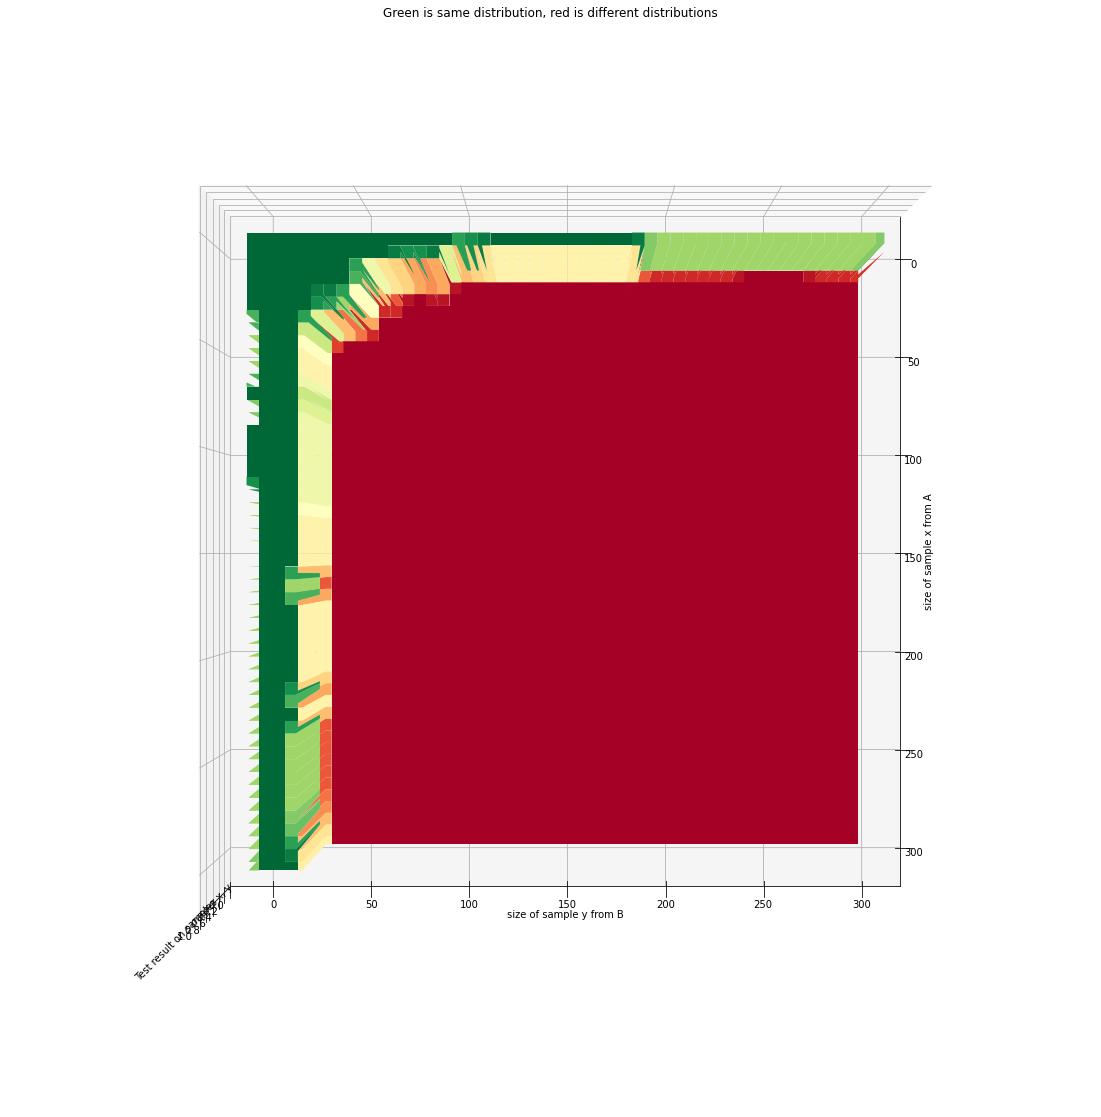
\includegraphics[width=\linewidth]{./img/hypothesis_test/appendix/ks_X_poisson_Y_student_t_shuffled.png}
  \caption{Poisson on X and Student T on Y axis}
\end{figure}
\clearpage
\subsection{Heatmaps of the naive method applied to samples of varying length from a single distribution}

\begin{figure}[htb]
  \centering
  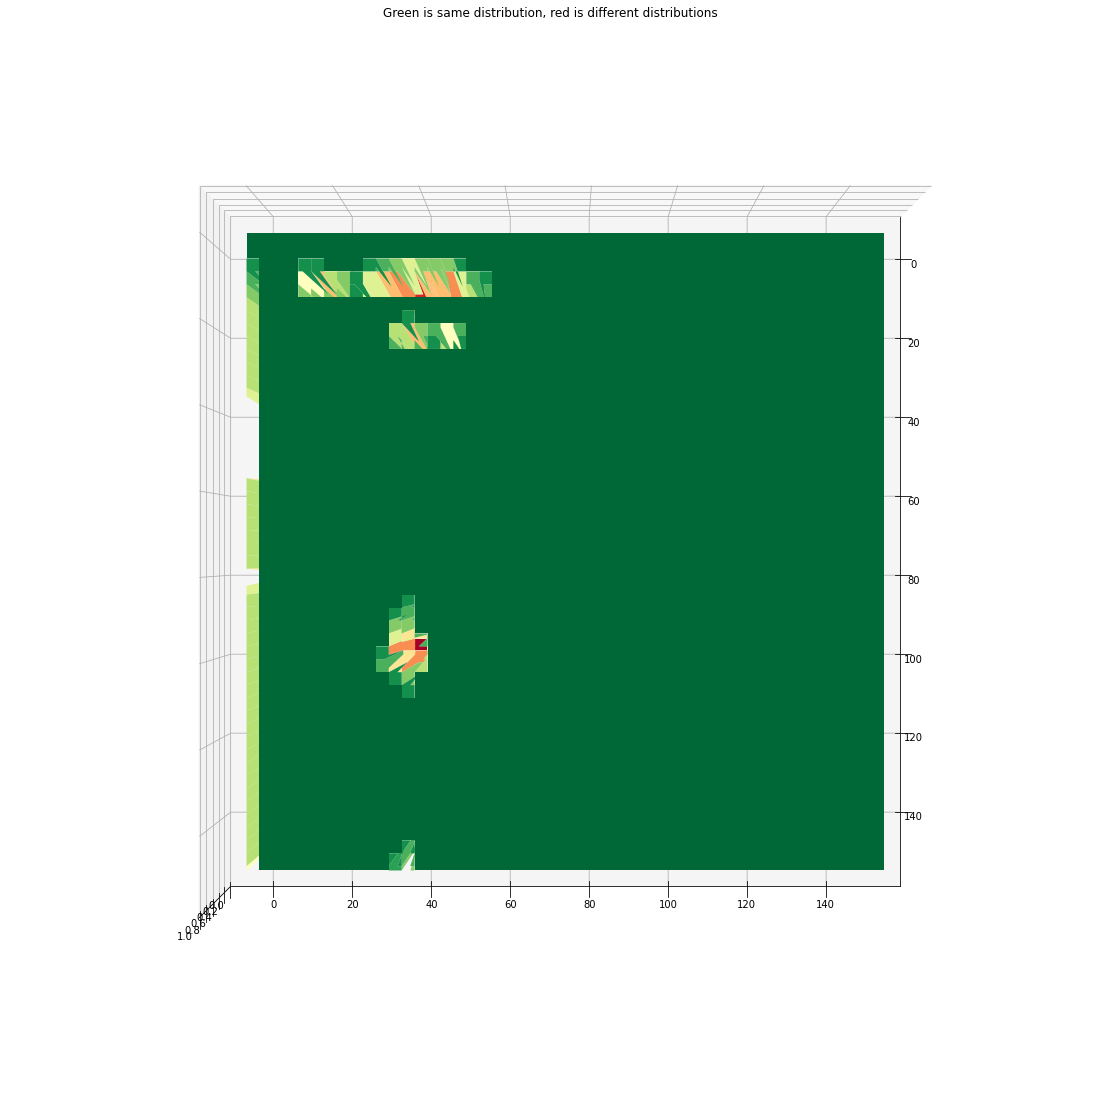
\includegraphics[width=\linewidth]{./img/hypothesis_test/appendix/naive_neg_bin.png}
  \caption{Negative Binomial}
\end{figure}
\clearpage
\begin{figure}[htb]
  \centering
  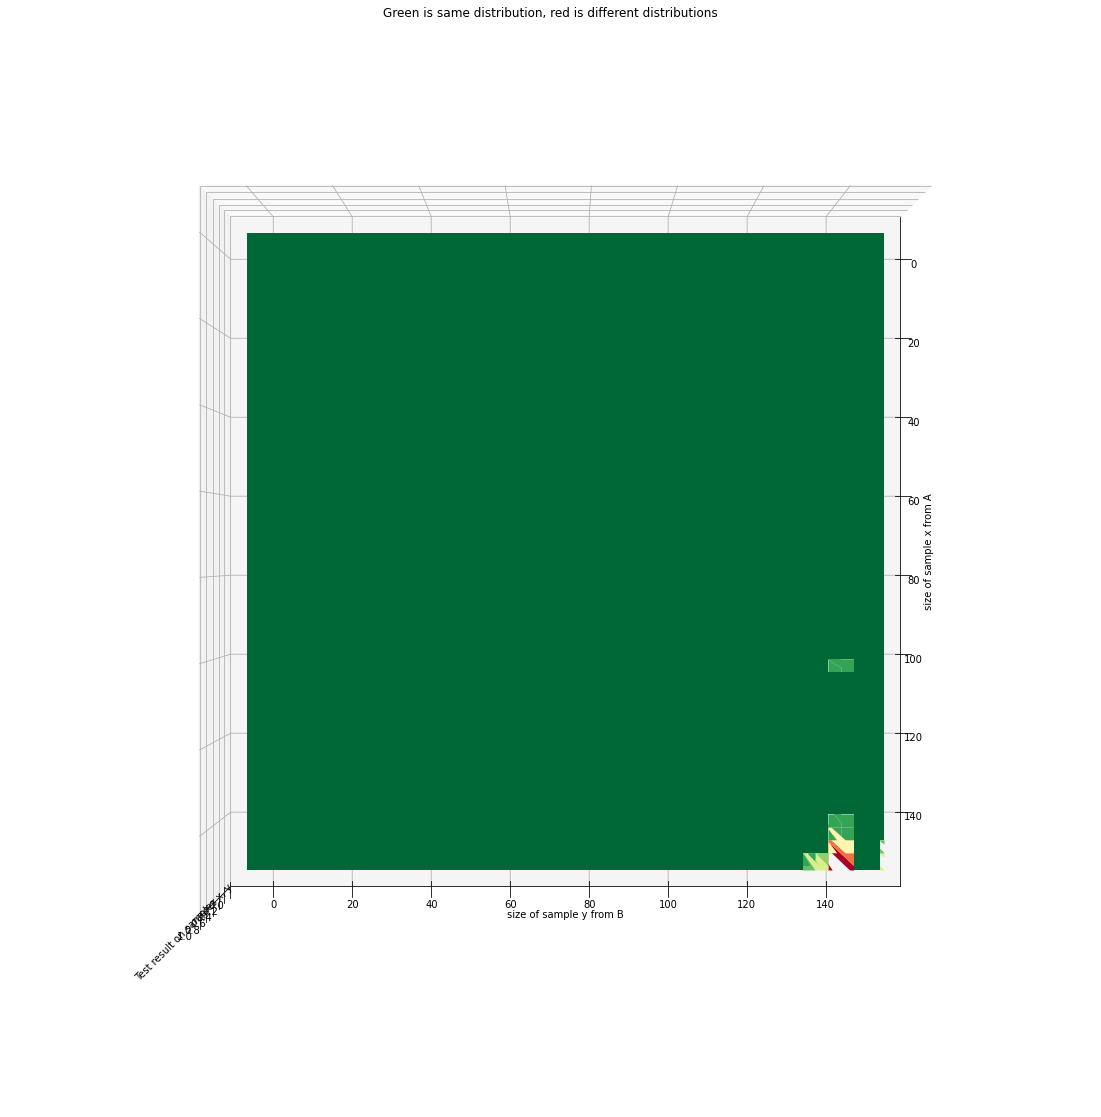
\includegraphics[width=\linewidth]{./img/hypothesis_test/appendix/naive_poisson.png}
  \caption{Poisson}
\end{figure}
\clearpage
\begin{figure}[htb]
  \centering
  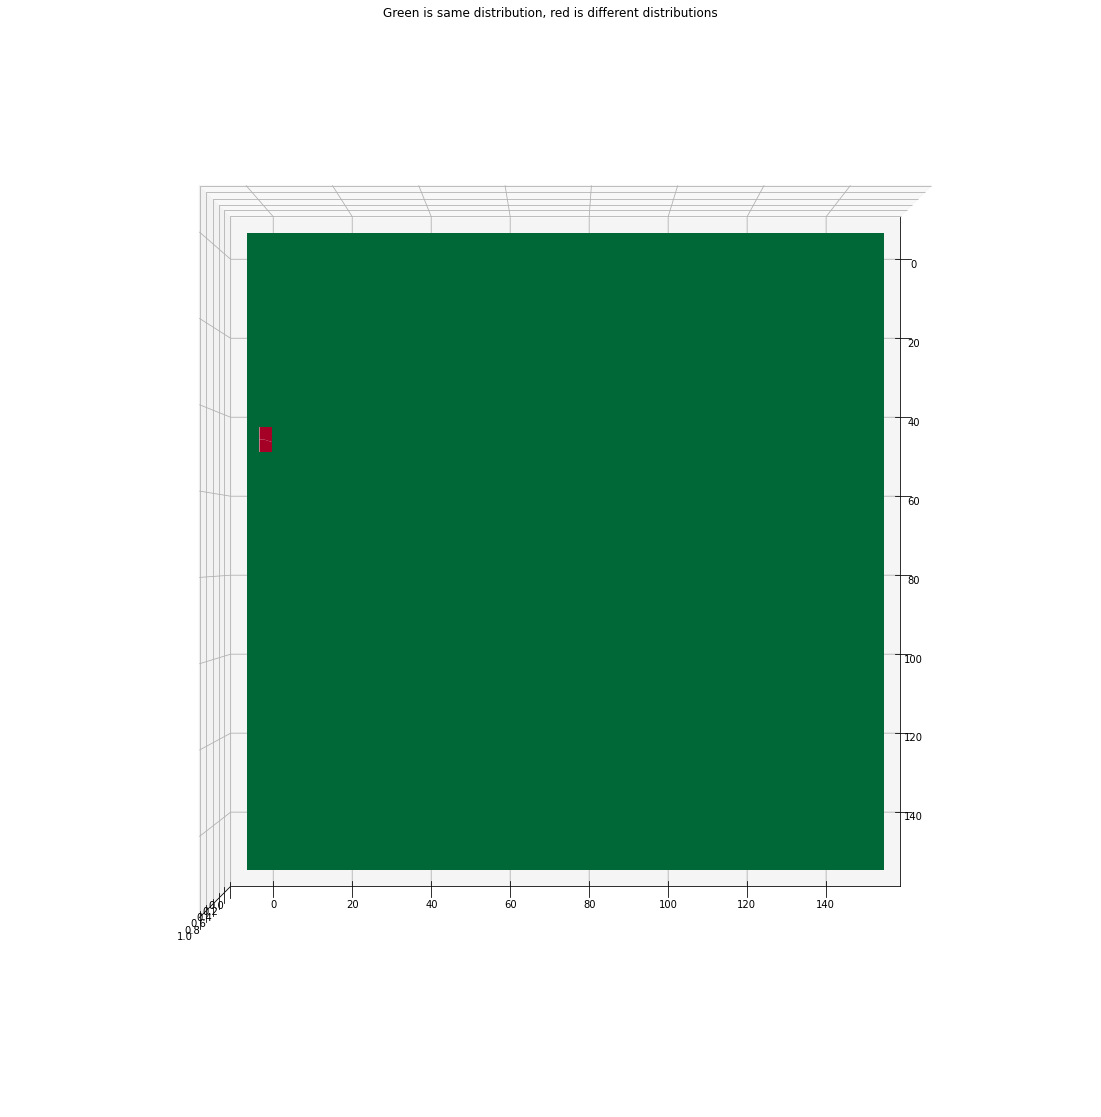
\includegraphics[width=\linewidth]{./img/hypothesis_test/appendix/naive_student_t.png}
  \caption{Student T}
\end{figure}
\clearpage
\subsection{Heatmaps of the naive method applied to samples of varying length from two independent distributions}

\begin{figure}[htb]
  \centering
  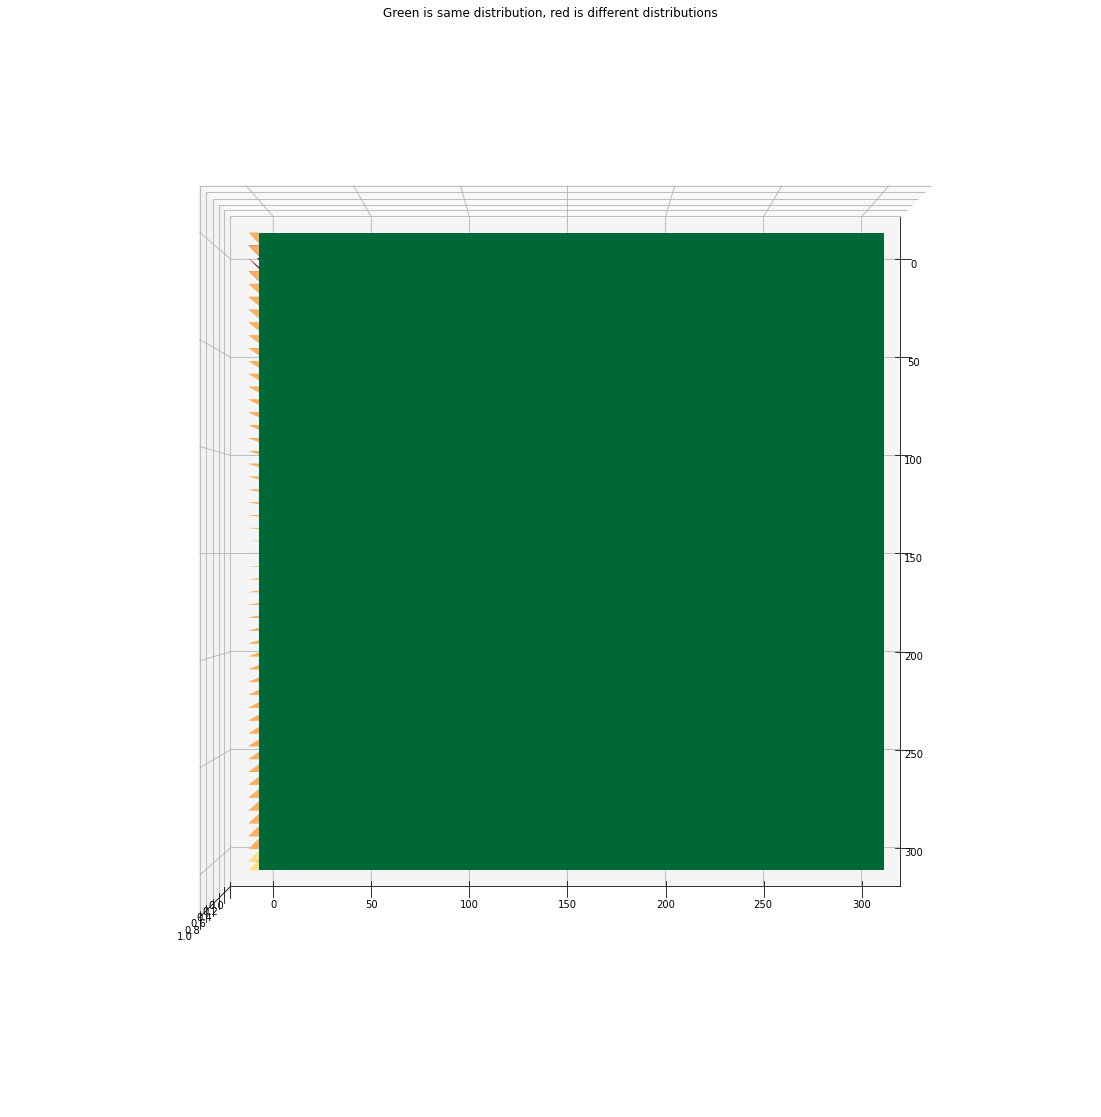
\includegraphics[width=\linewidth]{./img/hypothesis_test/appendix/naive_X_neg_bin_Y_student_t.png}
  \caption{Negative Binomial on X axis and Student T on Y axis}
\end{figure}
\clearpage
\begin{figure}[htb]
  \centering
  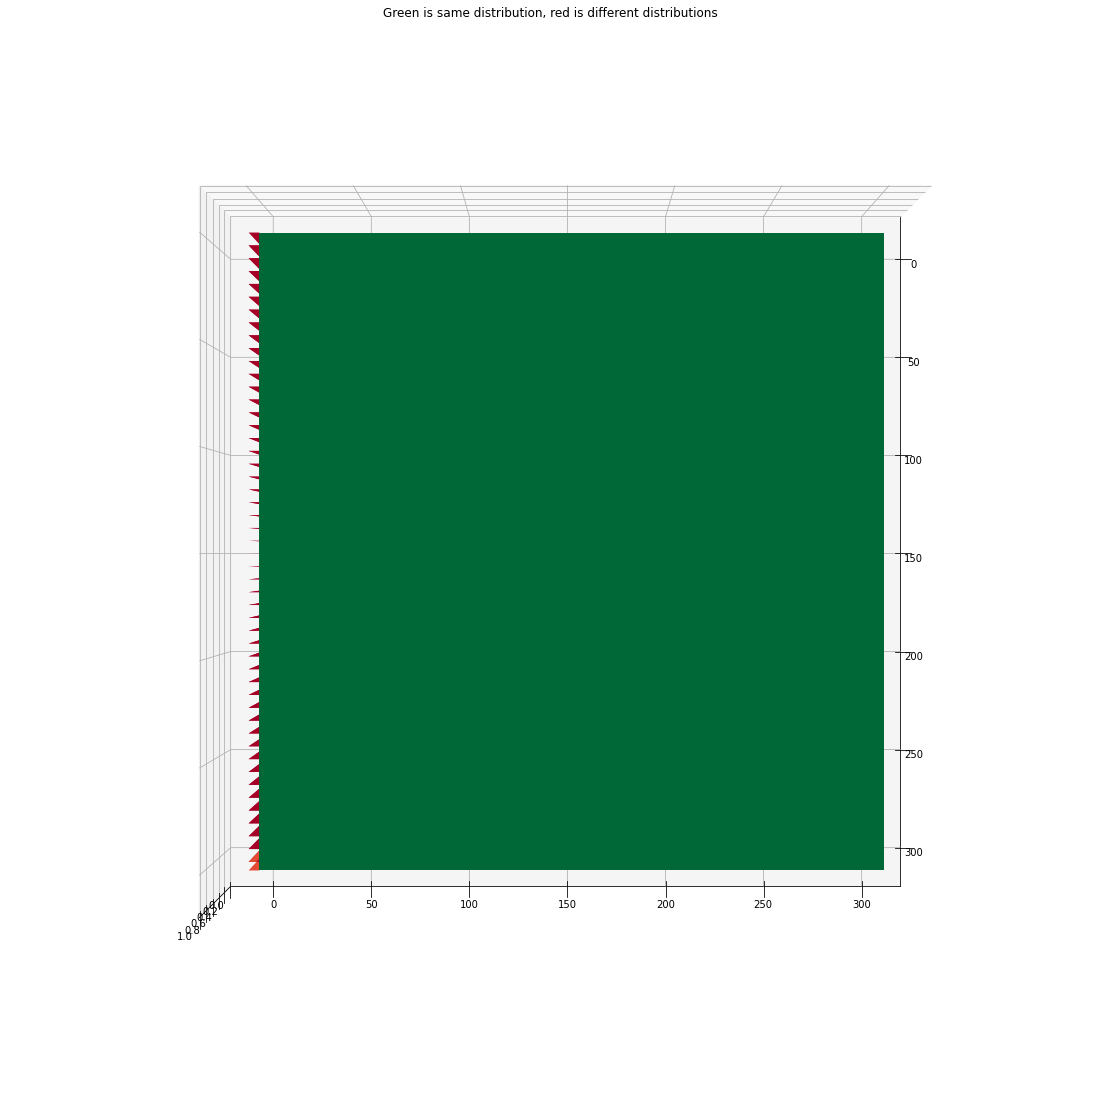
\includegraphics[width=\linewidth]{./img/hypothesis_test/appendix/naive_X_poisson_Y_neg_bin.png}
  \caption{Poisson on X axis and Negative Binomial on Y axis}
\end{figure}
\clearpage
\begin{figure}[htb]
  \centering
  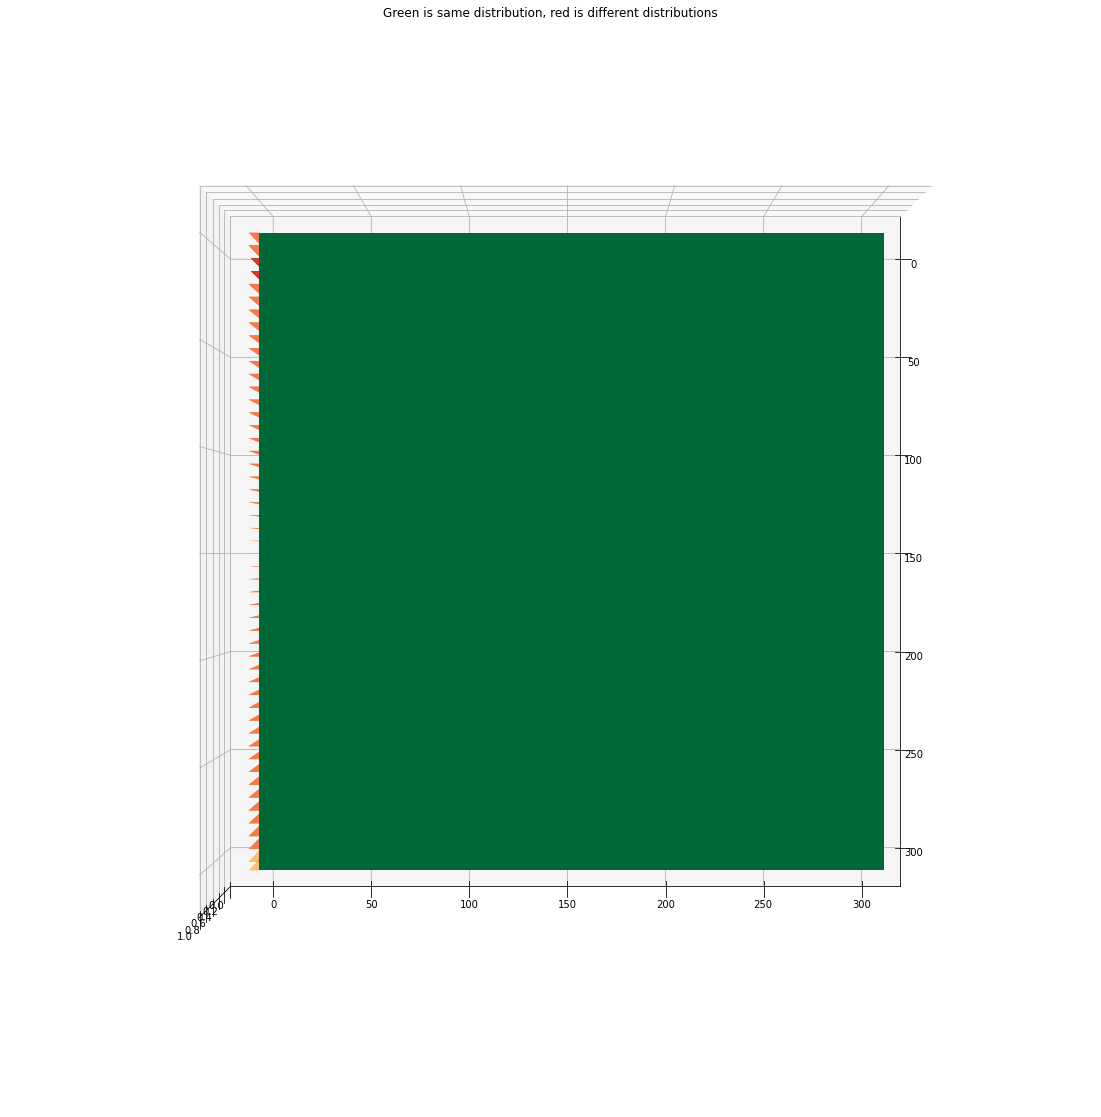
\includegraphics[width=\linewidth]{./img/hypothesis_test/appendix/naive_X_poisson_Y_student_t.png}
  \caption{Poisson on X and Student T on Y axis}
\end{figure}
\clearpage
\subsection{Heatmaps of the T-test applied to samples of varying length from a single distribution}

\begin{figure}[htb]
  \centering
  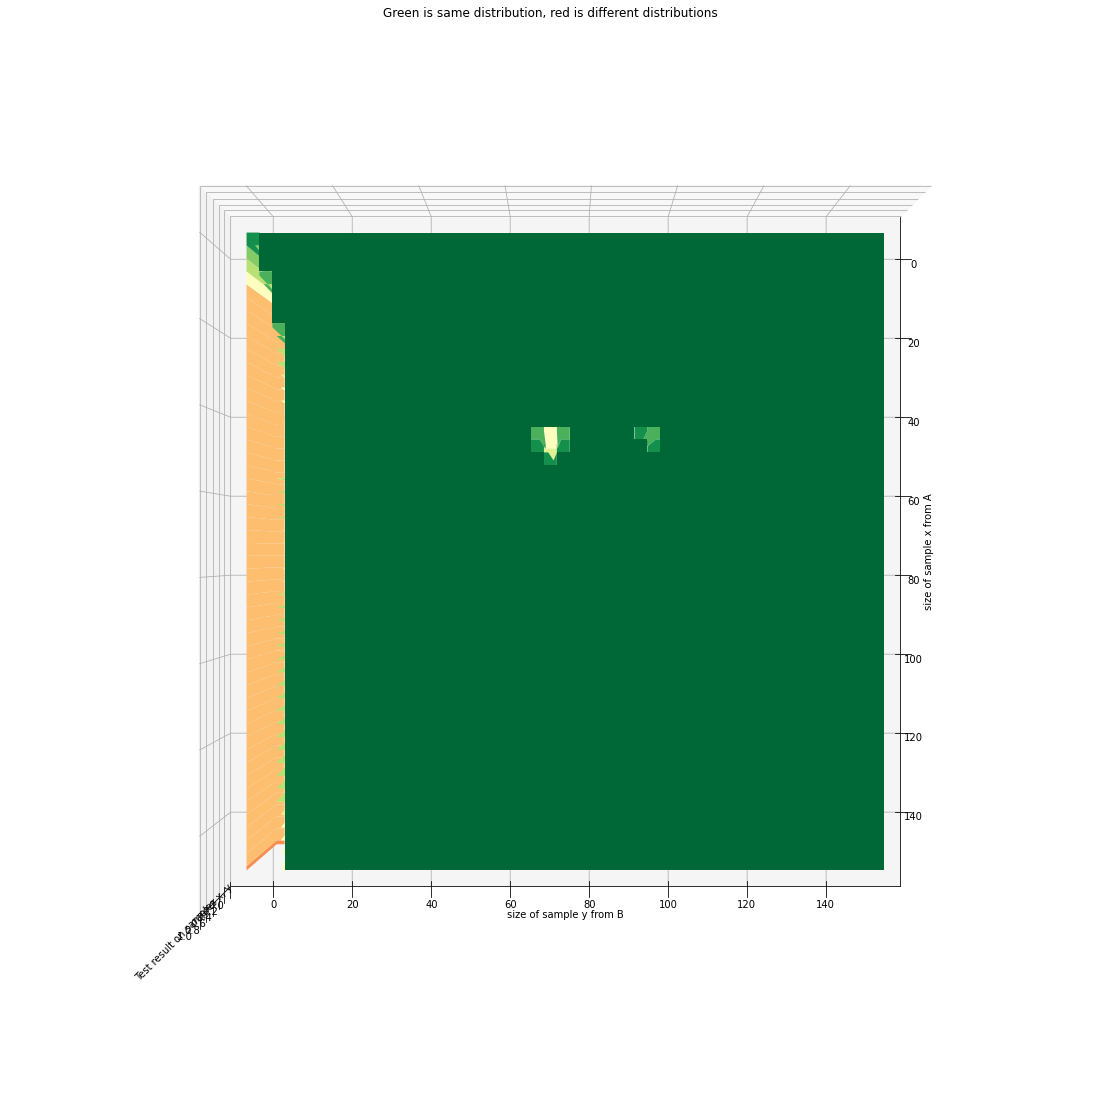
\includegraphics[width=\linewidth]{./img/hypothesis_test/appendix/ttest_neg_bin.png}
  \caption{Negative Binomial}
\end{figure}
\clearpage
\begin{figure}[htb]
  \centering
  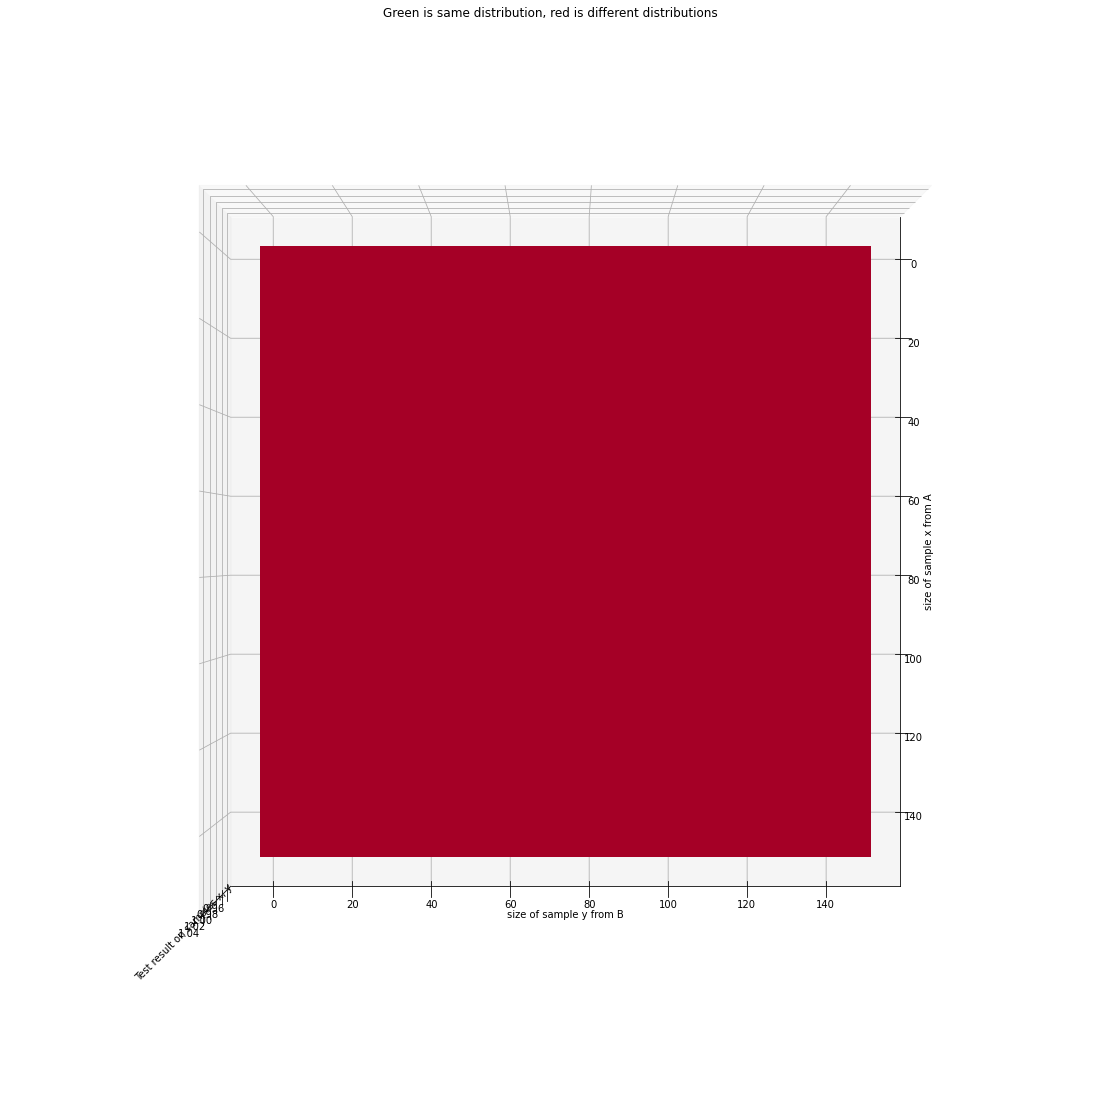
\includegraphics[width=\linewidth]{./img/hypothesis_test/appendix/ttest_poisson.png}
  \caption{Poisson}
\end{figure}
\clearpage
\begin{figure}[htb]
  \centering
  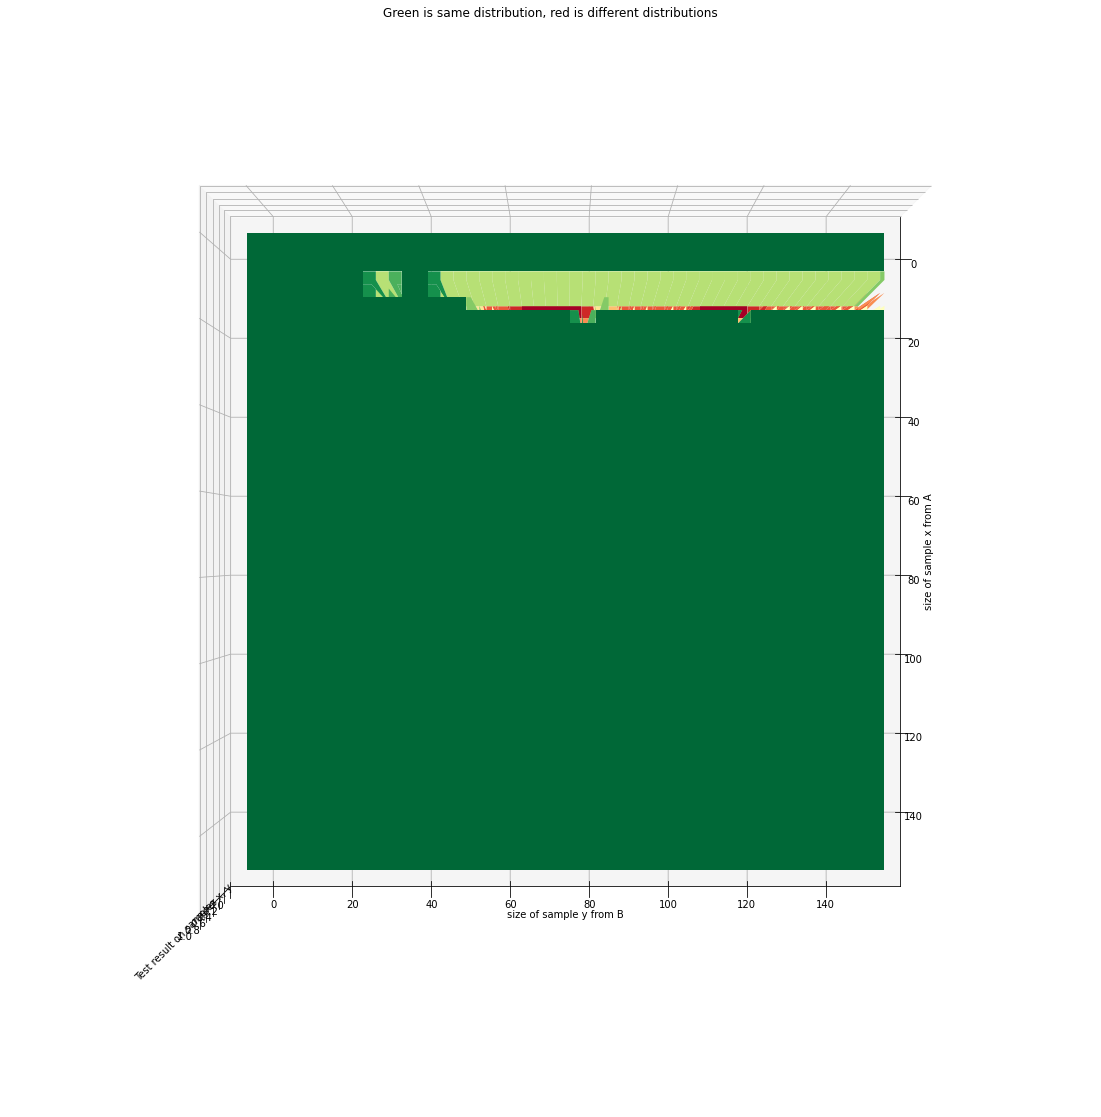
\includegraphics[width=\linewidth]{./img/hypothesis_test/appendix/ttest_student_t.png}
  \caption{Student T}
\end{figure}
\clearpage
\section{Dataset Plots and statistics}
\label{app:dataset_analysis}
\clearpage
\subsection{Electricity}
\begin{table}[htb]
  \begin{tabular}{||c | c c c c c c c c ||}
    \hline
    Dataset & Mean    & Series & Items    & Shortest & Longest & Min & Max      & Frequency \\ [0.5ex]
    \hline\hline
    train   & 2510.68 & 321    & 6755124  & 21044    & 21044   & 0.0 & 764000.0 & 1H        \\
    \hline
    test    & 2509.92 & 2247   & 47501580 & 21068    & 21212   & 0.0 & 764000.0 & 1H        \\
    \hline
  \end{tabular}
  \caption{Statistics of the Electricity dataset.}
\end{table}

\begin{figure}[htb]
  \centering
  \minipage{1.0\textwidth}
  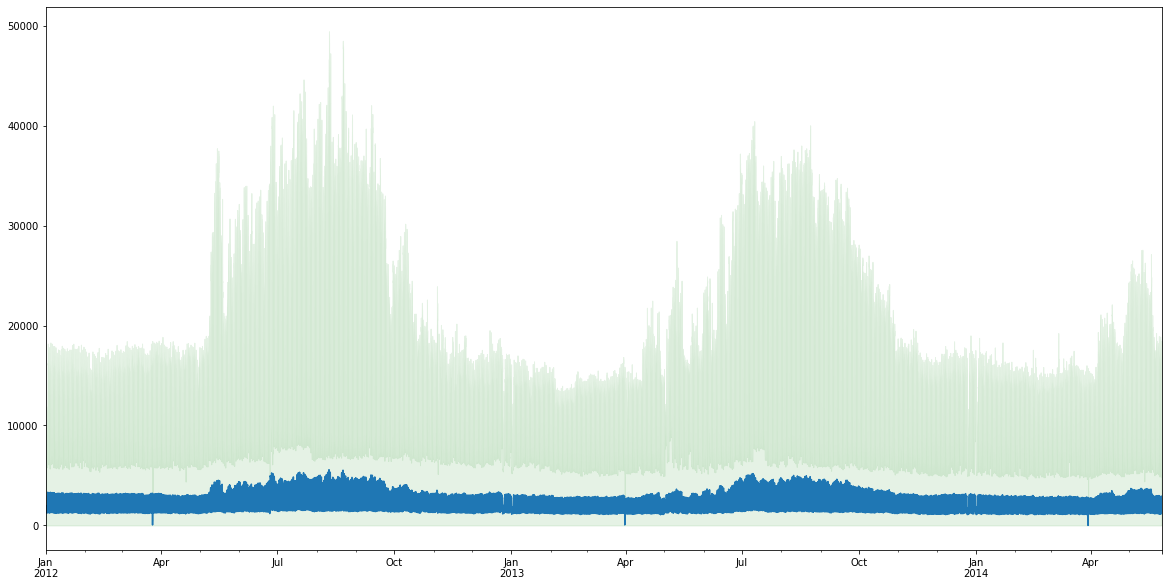
\includegraphics[width=\linewidth]{./img/electricity_plot.png}
  \caption{Plot over the average timeseries in the electricity dataset with one standard deviation shown in green. Only positive values are shown as the dataset is non-negative.}
  \label{fig:electricity_plot}
  \endminipage\hfill
\end{figure}

\begin{figure}[htb]
  \centering
  \minipage{1.0\textwidth}
  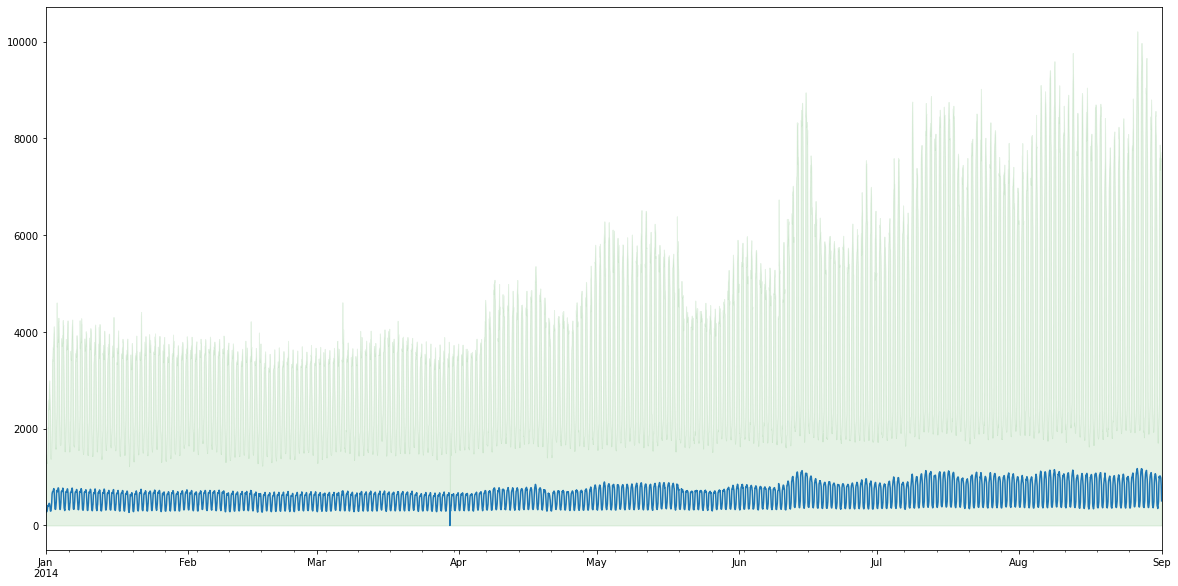
\includegraphics[width=\linewidth]{./img/electricity_no_negative.png}
  \caption{Zoomed version of \ref{fig:electricity_plot}}
  \label{fig:electricity_plot_zooomed}
  \endminipage\hfill
\end{figure}

\begin{figure}[htb]
  \centering
  \minipage{0.4\textwidth}
  \begin{center}
    \begin{tabular}{||c | c | c | c | c |}
      \hline
      statistic   & mean & deviation & max & min  \\
      \hline
      trend       & 0.65 & 0.17      & 1.0 & 0.09 \\
      \hline
      seasonality & 0.84 & 0.19      & 1.0 & 0.0  \\
      \hline
      \hline
    \end{tabular}
    \caption{Strength of trend and seasonality of the Electricity dataset}
  \end{center}
  \endminipage\hfill
  \minipage{0.45\textwidth}
  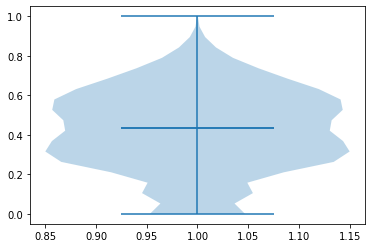
\includegraphics[width=\linewidth]{./img/electricity_violin.png}
  \caption{Scaled violin plot of the electricity dataset.}
  \label{fig:electricity_violin}
  \endminipage\hfill
\end{figure}

\clearpage
\subsection{Exchange Rate}

\begin{table}[htb]
  \begin{tabular}{||c | c c c c c c c c ||}
    \hline
    Dataset & Mean & Series & Items  & Shortest & Longest & Min  & Max  & Frequency \\ [0.5ex]
    \hline\hline
    train   & 0.68 & 8      & 48568  & 6071     & 6071    & 0.01 & 2.11 & 1B        \\
    \hline
    test    & 0.68 & 40     & 246440 & 6101     & 6221    & 0.01 & 2.11 & 1B        \\
    \hline
  \end{tabular}
  \caption{Statistics of the Exchange Rate dataset}
\end{table}

\begin{figure}[htb]
  \centering
  \minipage{1.0\textwidth}
  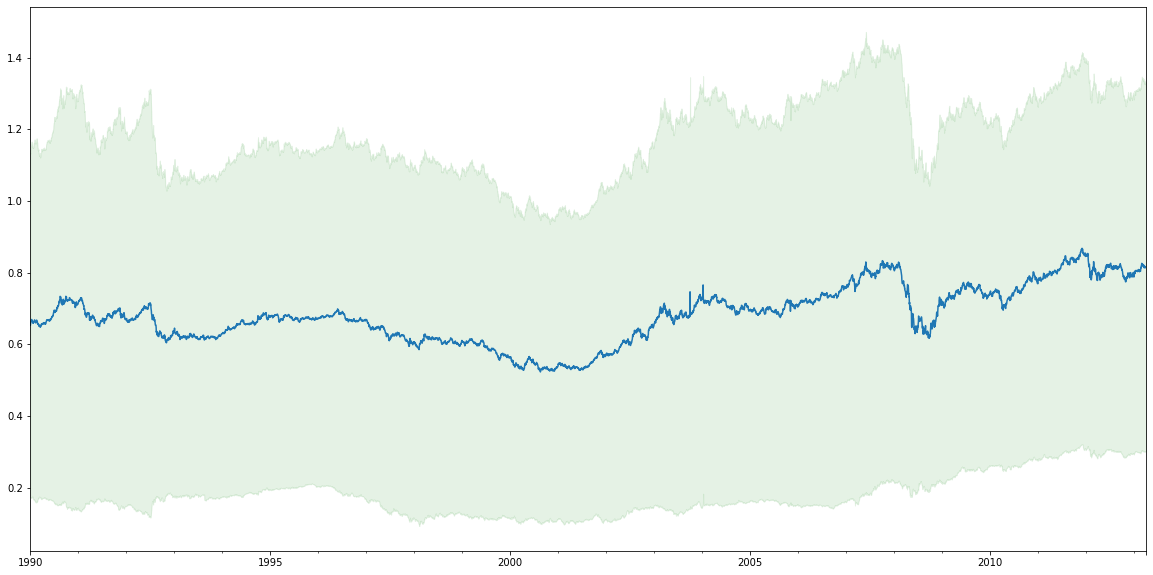
\includegraphics[width=\linewidth]{./img/exchange_rate_plot.png}
  \caption{Plot over the average timeseries in the exchange rate dataset with one standard deviation shown in green. Only positive values are shown as the dataset is non-negative.}
  \label{fig:exchange_rate_plot}
  \endminipage\hfill
\end{figure}

\begin{figure}[htb]
  \centering
  \minipage{0.4\textwidth}
  \begin{center}
    \begin{tabular}{||c | c | c | c | c |}
      \hline
      statistic   & mean & deviation & max  & min  \\
      \hline
      trend       & 1.0  & 0.0       & 1.0  & 0.99 \\
      \hline
      seasonality & 0.12 & 0.30      & 0.90 & 0.0  \\
      \hline
      \hline
    \end{tabular}
    \caption{Strength of trend and seasonality of the exchange rate dataset}
  \end{center}
  \endminipage\hfill
  \minipage{0.45\textwidth}
  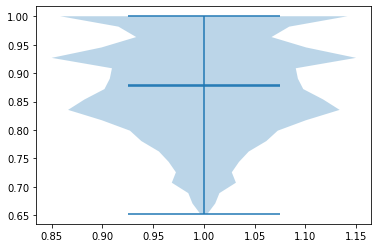
\includegraphics[width=\linewidth]{./img/exchange_rate_violin.png}
  \caption{Scaled violin plot of the exchange rate dataset.}
  \label{fig:exchange_rate_violin}
  \endminipage\hfill
\end{figure}

\clearpage
\subsection{Solar Energy}


\begin{table}[htb]
  \begin{tabular}{||c | c c c c c c c c ||}
    \hline
    Dataset & Mean  & Series & Items   & Shortest & Longest & Min & Max    & Frequency \\ [0.5ex]
    \hline\hline
    train   & 40.35 & 137    & 960233  & 7009     & 7009    & 0.0 & 509.05 & 10min     \\
    \hline
    test    & 40.25 & 959    & 6813695 & 7033     & 7177    & 0.0 & 509.05 & 10min     \\
    \hline
  \end{tabular}
  \caption{Statistics of the Solar Energy dataset}
\end{table}


\begin{figure}[htb]
  \centering
  \minipage{1.0\textwidth}
  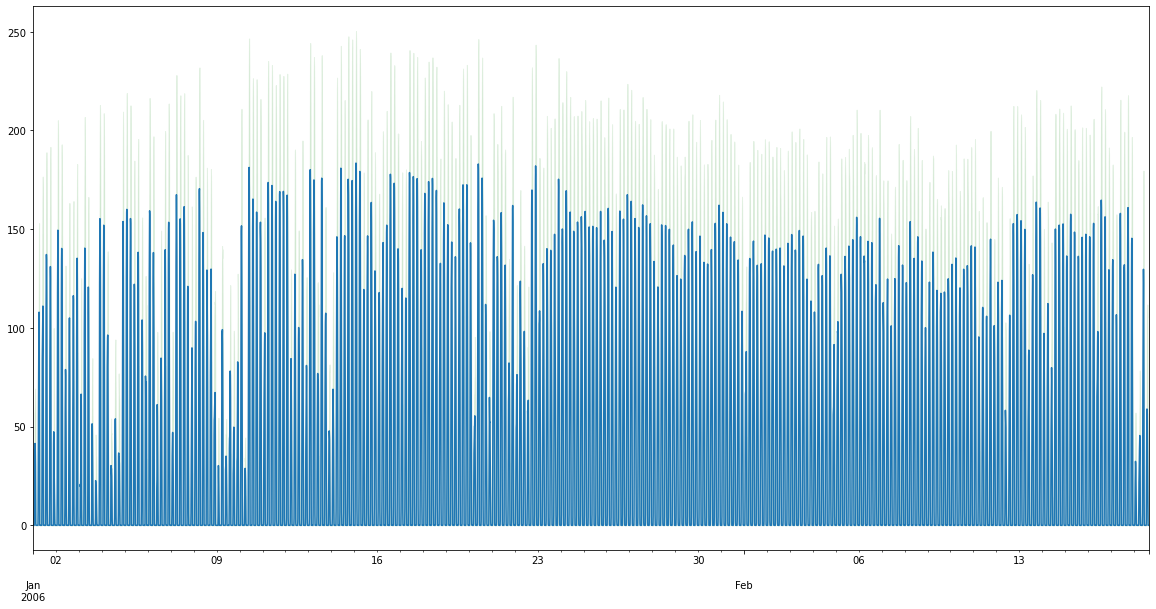
\includegraphics[width=\linewidth]{./img/solar-energy_plot.png}
  \caption{Plot over the average timeseries in the solar energy dataset with one standard deviation shown in green. Only positive values are shown as the dataset is non-negative.}
  \label{fig:solar-energy_plot}
  \endminipage\hfill
\end{figure}

\begin{figure}[htb]
  \centering
  \minipage{0.4\textwidth}
  \begin{center}
    \begin{tabular}{||c | c | c | c | c |}
      \hline
      statistic   & mean & deviation & max  & min  \\
      \hline
      trend       & 0.09 & 0.03      & 0.15 & 0.0  \\
      \hline
      seasonality & 0.84 & 0.02      & 0.87 & 0.79 \\
      \hline
      \hline
    \end{tabular}
    \caption{Strength of trend and seasonality of the solar-energy dataset}
  \end{center}
  \endminipage\hfill
  \minipage{0.45\textwidth}
  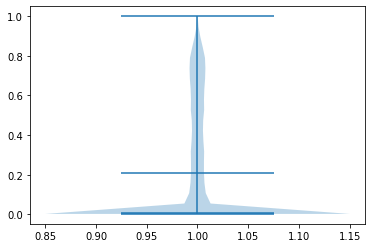
\includegraphics[width=\linewidth]{./img/solar-energy_violin.png}
  \caption{Scaled violin plot of the solar energy dataset.}
  \label{fig:solar-energy_violin}
  \endminipage\hfill
\end{figure}

\clearpage
\subsection{Traffic}

\begin{table}[htb]
  \begin{tabular}{||c | c c c c c c c c ||}
    \hline
    Dataset & Mean & Series & Items    & Shortest & Longest & Min & Max  & Frequency \\ [0.5ex]
    \hline\hline
    train   & 0.06 & 862    & 12099032 & 14036    & 14036   & 0.0 & 0.72 & H         \\
    \hline
    test    & 0.06 & 6034   & 85272488 & 14060    & 14204   & 0.0 & 0.72 & H         \\
    \hline
  \end{tabular}
  \caption{Statistics of the Traffic dataset}
\end{table}

\begin{figure}[htb]
  \centering
  \minipage{1.0\textwidth}
  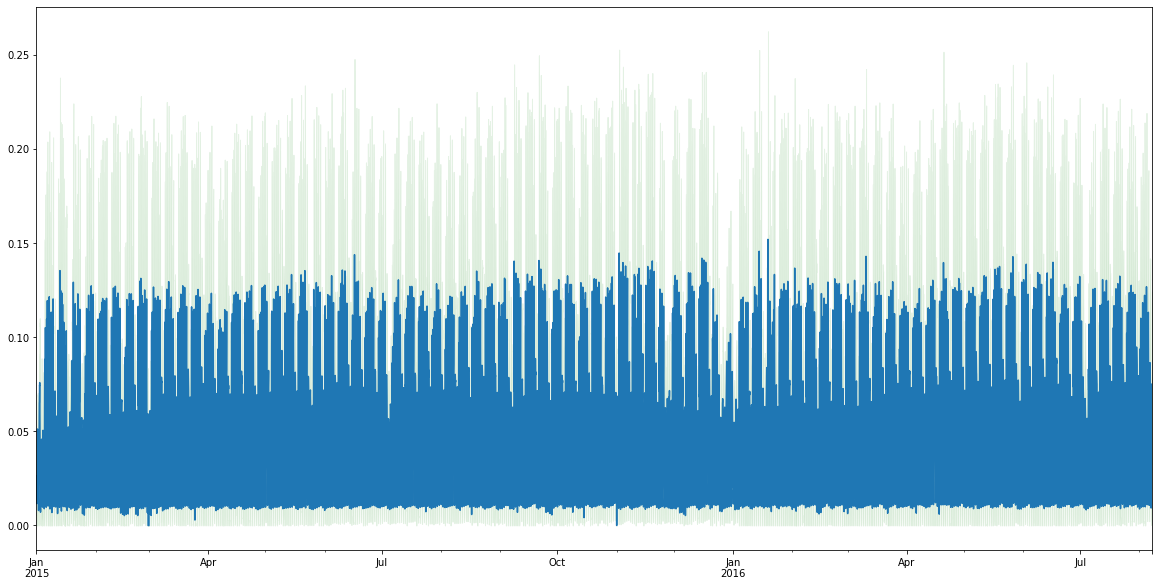
\includegraphics[width=\linewidth]{./img/traffic_plot.png}
  \caption{Plot over the average timeseries in the traffic dataset with one standard deviation shown in green. Only positive values are shown as the dataset is non-negative.}
  \label{fig:traffic_plot}
  \endminipage\hfill
\end{figure}

\begin{figure}[htb]
  \centering
  \minipage{0.4\textwidth}
  \begin{center}
    \begin{tabular}{||c | c | c | c | c |}
      \hline
      statistic   & mean & deviation & max  & min  \\
      \hline
      trend       & 0.16 & 0.12      & 0.79 & 0.0  \\
      \hline
      seasonality & 0.67 & 0.10      & 0.93 & 0.12 \\
      \hline
      \hline
    \end{tabular}
    \caption{Strength of trend and seasonality of the traffic dataset}
  \end{center}
  \endminipage\hfill
  \minipage{0.45\textwidth}
  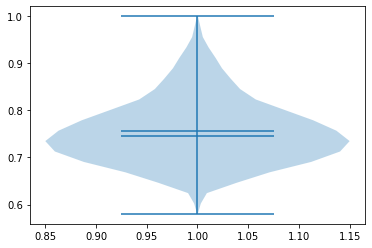
\includegraphics[width=\linewidth]{./img/traffic_violin.png}
  \caption{Scaled violin plot of the traffic dataset.}
  \label{fig:traffic_violin}
  \endminipage\hfill
\end{figure}

\clearpage
\subsection{Exchange Rate NIPS}
\begin{table}[htb]
  \begin{tabular}{||c | c c c c c c c c ||}
    \hline
    Dataset & Mean & Series & Items  & Shortest & Longest & Min  & Max  & Frequency \\ [0.5ex]
    \hline\hline
    train   & 0.68 & 8      & 48568  & 6071     & 6071    & 0.01 & 2.11 & B         \\
    \hline
    test    & 0.68 & 40     & 246440 & 6101     & 6221    & 0.01 & 2.11 & B         \\
    \hline
  \end{tabular}
  \caption{Statistics of the Exchange Rate NIPS dataset}
\end{table}

\begin{figure}[htb]
  \centering
  \minipage{1.0\textwidth}
  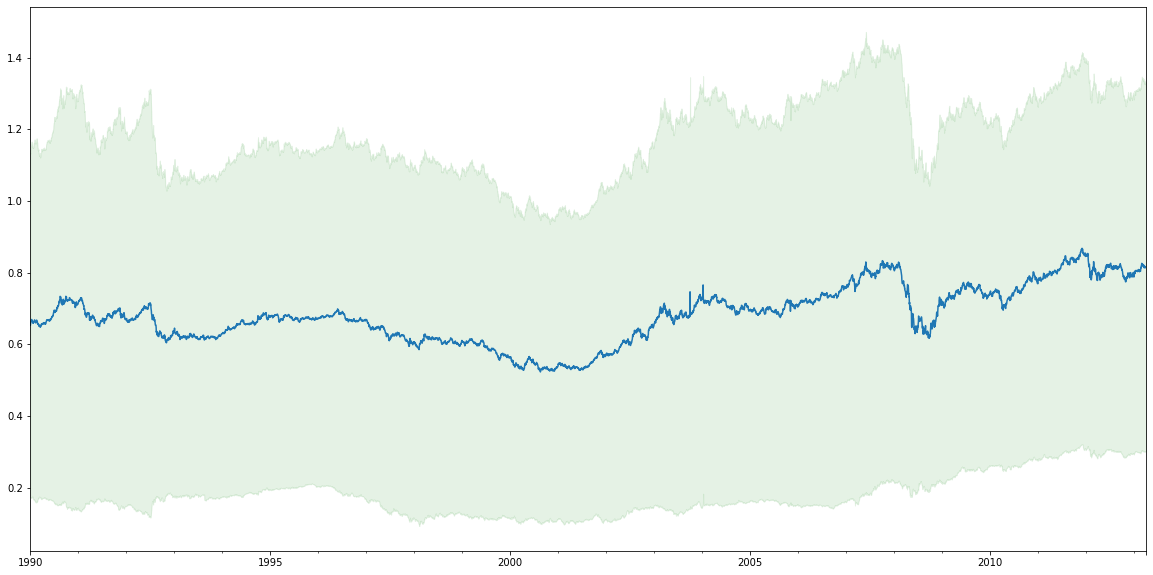
\includegraphics[width=\linewidth]{./img/exchange_rate_nips_plot.png}
  \caption{Plot over the average timeseries in the exchange rate nips dataset with one standard deviation shown in green. Only positive values are shown as the dataset is non-negative.}
  \label{fig:exchange_rate_nips_plot}
  \endminipage\hfill
\end{figure}

\begin{figure}[htb]
  \centering
  \minipage{0.4\textwidth}
  \begin{center}
    \begin{tabular}{||c | c | c | c | c |}
      \hline
      statistic   & mean & deviation & max  & min  \\
      \hline
      trend       & 1.0  & 0.0       & 1.0  & 0.99 \\
      \hline
      seasonality & 0.12 & 0.30      & 0.90 & 0.0  \\
      \hline
      \hline
    \end{tabular}
    \caption{Strength of trend and seasonality of the exchange rate nips dataset}
  \end{center}
  \endminipage\hfill
  \minipage{0.45\textwidth}
  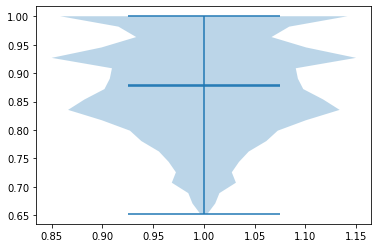
\includegraphics[width=\linewidth]{./img/exchange_rate_nips_violin.png}
  \caption{Scaled violin plot of the exchange rate nips dataset.}
  \label{fig:exchange_rate_nips_violin}
  \endminipage\hfill
\end{figure}

\clearpage
\subsection{Electricity NIPS}
\begin{table}[htb]
  \begin{tabular}{||c | c c c c c c c c ||}
    \hline
    Dataset & Mean   & Series & Items    & Shortest & Longest & Min & Max      & Frequency \\ [0.5ex]
    \hline\hline
    train   & 607.95 & 370    & 2142282  & 1081     & 5833    & 0.0 & 168100.0 & H         \\
    \hline
    test    & 652.36 & 2590   & 10340239 & 1105     & 4000    & 0.0 & 168100.0 & H         \\
    \hline
  \end{tabular}
  \caption{Statistics of the Electricity NIPS dataset.}
\end{table}

\begin{figure}[htb]
  \centering
  \minipage{1.0\textwidth}
  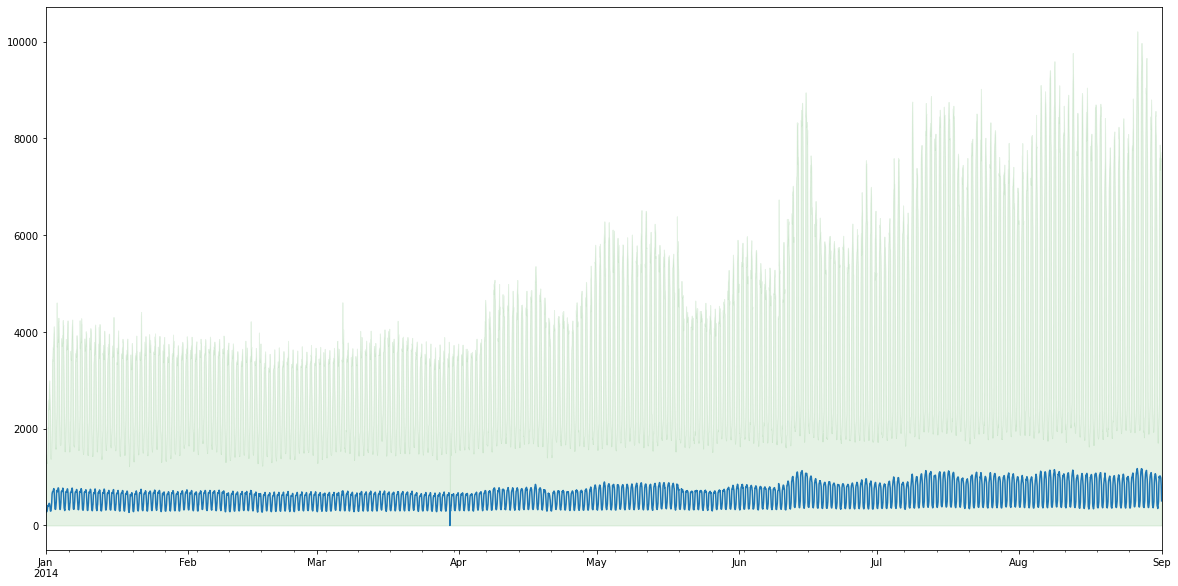
\includegraphics[width=\linewidth]{./img/electricity_nips_plot.png}
  \caption{Plot over the average timeseries in the electricity nips dataset with one standard deviation shown in green. Only positive values are shown as the dataset is non-negative.}
  \label{fig:electricity_nips_plot}
  \endminipage\hfill
\end{figure}

\begin{figure}[htb]
  \centering
  \minipage{0.4\textwidth}
  \begin{center}
    \begin{tabular}{||c | c | c | c | c |}
      \hline
      statistic   & mean & deviation & max & min \\
      \hline
      trend       & 0.54 & 0.20      & 1.0 & 0.0 \\
      \hline
      seasonality & 0.86 & 0.16      & 1.0 & 0.0 \\
      \hline
      \hline
    \end{tabular}
    \caption{Strength of trend and seasonality of the electricity nips dataset}
  \end{center}
  \endminipage\hfill
  \minipage{0.45\textwidth}
  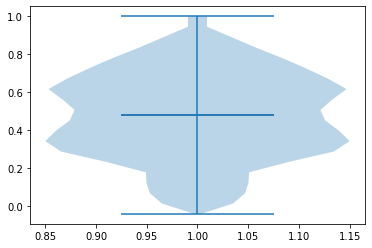
\includegraphics[width=\linewidth]{./img/electricity_nips_violin.png}
  \caption{Scaled violin plot of the electricity nips dataset.}
  \label{fig:electricity_nips_violin}
  \endminipage\hfill
\end{figure}

\clearpage
\subsection{Solar Energy NIPS}
\begin{table}[htb]
  \begin{tabular}{||c | c c c c c c c c ||}
    \hline
    Dataset & Mean  & Series & Items   & Shortest & Longest & Min  & Max    & Frequency \\ [0.5ex]
    \hline\hline
    train   & 40.35 & 137    & 960233  & 7009     & 7009    & 0.00 & 509.05 & H         \\
    \hline
    test    & 40.25 & 959    & 6813695 & 7033     & 7177    & 0.00 & 509.05 & H         \\
    \hline
  \end{tabular}
  \caption{Statistics of the Solar Energy NIPS dataset}
\end{table}

\begin{figure}[htb]
  \centering
  \minipage{1.0\textwidth}
  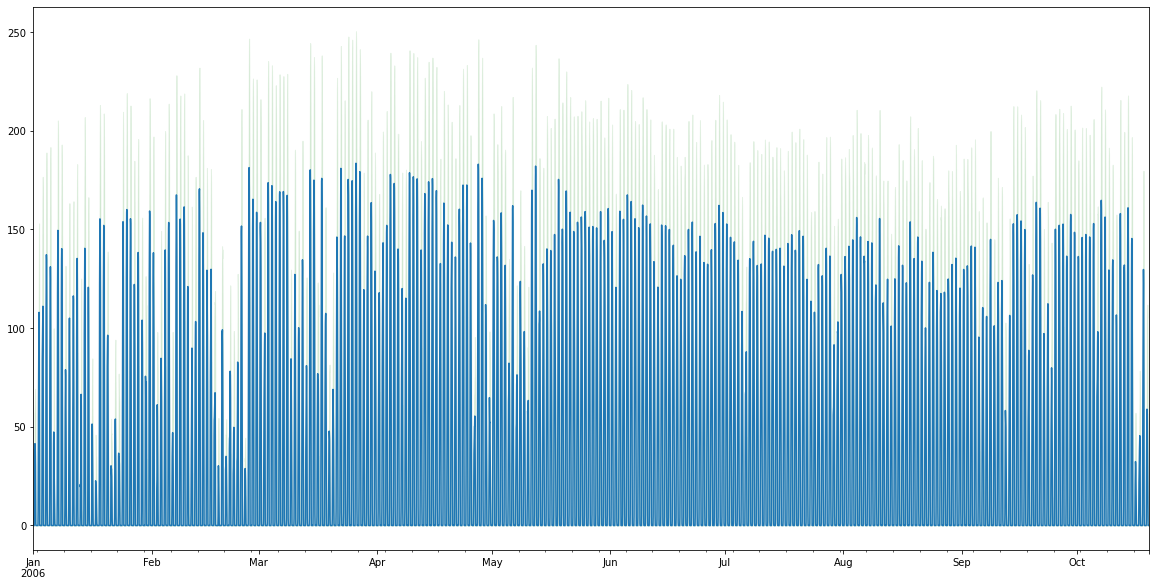
\includegraphics[width=\linewidth]{./img/solar_nips_plot.png}
  \caption{Plot over the average timeseries in the solar nips dataset with one standard deviation shown in green. Only positive values are shown as the dataset is non-negative.}
  \label{fig:solar_nips_plot}
  \endminipage\hfill
\end{figure}

\begin{figure}[htb]
  \centering
  \minipage{0.4\textwidth}
  \begin{center}
    \begin{tabular}{||c | c | c | c | c |}
      \hline
      statistic   & mean & deviation & max  & min  \\
      \hline
      trend       & 0.17 & 0.02      & 0.24 & 0.11 \\
      \hline
      seasonality & 0.86 & 0.02      & 0.89 & 0.80 \\
      \hline
      \hline
    \end{tabular}
    \caption{Strength of trend and seasonality of the solar nips dataset}
  \end{center}
  \endminipage\hfill
  \minipage{0.45\textwidth}
  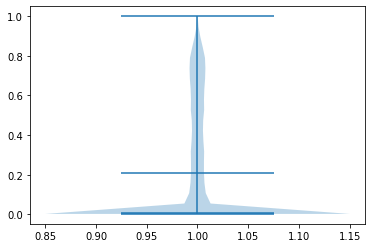
\includegraphics[width=\linewidth]{./img/solar_nips_violin.png}
  \caption{Scaled violin plot of the solar nips dataset.}
  \label{fig:solar_nips_violin}
  \endminipage\hfill
\end{figure}


\clearpage
\subsection{Traffic NIPS}
\begin{table}[htb]
  \begin{tabular}{||c | c c c c c c c c ||}
    \hline
    Dataset & Mean & Series & Items    & Shortest & Longest & Min  & Max  & Frequency \\ [0.5ex]
    \hline\hline
    train   & 0.05 & 963    & 3852963  & 4001     & 4001    & 0.00 & 1.00 & H         \\
    \hline
    test    & 0.05 & 6741   & 26964000 & 4000     & 4000    & 0.00 & 1.00 & H         \\
    \hline
  \end{tabular}
  \caption{Statistics of the Traffic NIPS dataset}
\end{table}


\begin{figure}[htb]
  \centering
  \minipage{1.0\textwidth}
  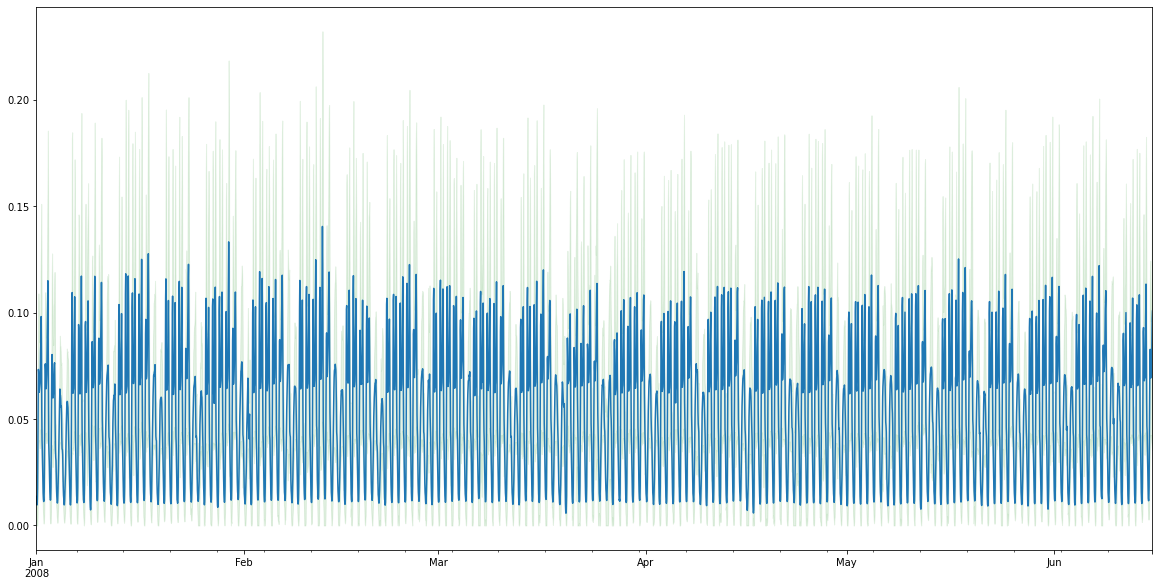
\includegraphics[width=\linewidth]{./img/traffic_nips_plot.png}
  \caption{Plot over the average timeseries in the traffic nips dataset with one standard deviation shown in green. Only positive values are shown as the dataset is non-negative.}
  \label{fig:traffic_nips_plot}
  \endminipage\hfill
\end{figure}

\begin{figure}[htb]
  \centering
  \minipage{0.4\textwidth}
  \begin{center}
    \begin{tabular}{||c | c | c | c | c |}
      \hline
      statistic   & mean & deviation & max  & min \\
      \hline
      trend       & 0.29 & 0.18      & 0.87 & 0.0 \\
      \hline
      seasonality & 0.76 & 0.12      & 0.94 & 0.0 \\
      \hline
      \hline
    \end{tabular}
    \caption{Strength of trend and seasonality of the traffic nips dataset}
  \end{center}
  \endminipage\hfill
  \minipage{0.45\textwidth}
  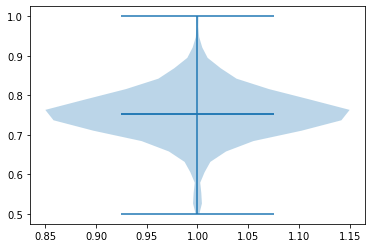
\includegraphics[width=\linewidth]{./img/traffic_nips_violin.png}
  \caption{Scaled violin plot of the traffic nips dataset.}
  \label{fig:traffic_nips_violin}
  \endminipage\hfill
\end{figure}
\clearpage
\subsection{Wiki Rolling NIPS}

\begin{table}[htb]
  \begin{tabular}{||c | c c c c c c c c ||}
    \hline
    Dataset & Mean    & Series & Items    & Shortest & Longest & Min  & Max        & Frequency \\ [0.5ex]
    \hline\hline
    train   & 3720.54 & 9535   & 7551720  & 792      & 792     & 0.00 & 7752515.00 & D         \\
    \hline
    test    & 3663.55 & 47675  & 40619100 & 792      & 912     & 0.00 & 7752515.00 & D         \\
    \hline
  \end{tabular}
  \caption{Statistics of the Wiki Rolling NIPS dataset}
\end{table}


\begin{figure}[htb]
  \centering
  \minipage{1.0\textwidth}
  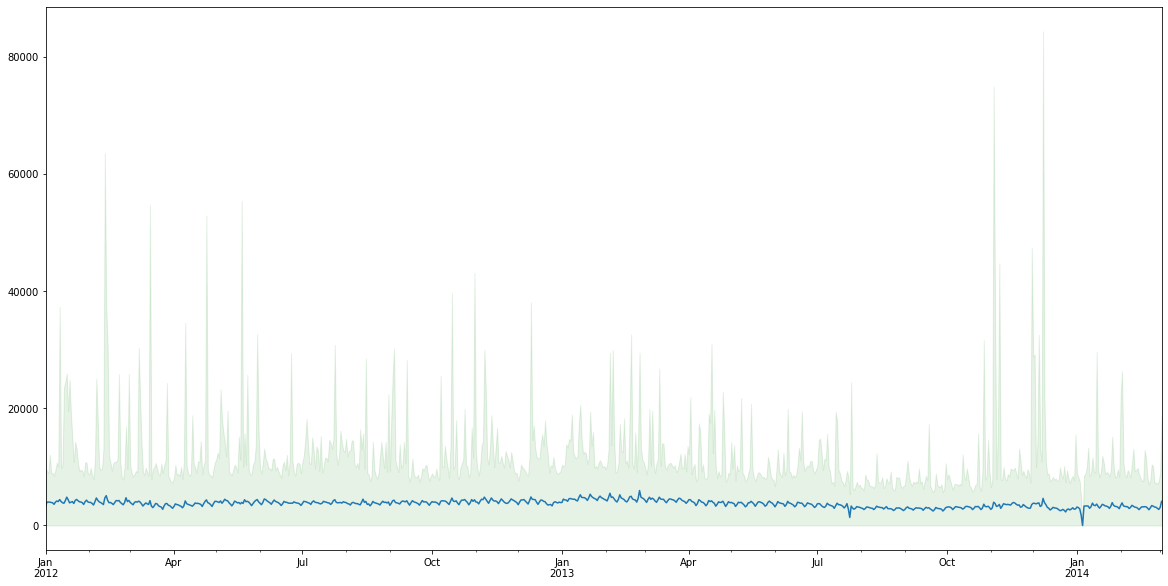
\includegraphics[width=\linewidth]{./img/wiki-rolling_nips_plot.png}
  \caption{Plot over the average timeseries in the wiki-rolling nips dataset with one standard deviation shown in green. Only positive values are shown as the dataset is non-negative.}
  \label{fig:wiki-rolling_nips_plot}
  \endminipage\hfill
\end{figure}

\begin{figure}[htb]
  \centering
  \minipage{0.4\textwidth}
  \begin{center}
    \begin{tabular}{||c | c | c | c | c |}
      \hline
      statistic   & mean & deviation & max & min \\
      \hline
      trend       & 0.53 & 0.27      & 1.0 & 0.0 \\
      \hline
      seasonality & 0.23 & 0.26      & 1.0 & 0.0 \\
      \hline
      \hline
    \end{tabular}
    \caption{Strength of trend and seasonality of the wiki-rolling nips dataset}
  \end{center}
  \endminipage\hfill
  \minipage{0.45\textwidth}
  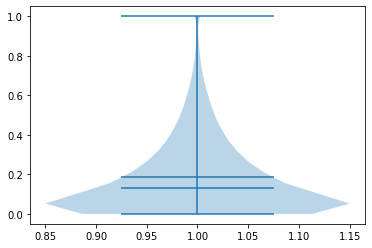
\includegraphics[width=\linewidth]{./img/wiki-rolling_nips_violin.png}
  \caption{Scaled violin plot of the wiki-rolling nips dataset.}
  \label{fig:wiki-rolling_nips_violin}
  \endminipage\hfill
\end{figure}

\clearpage
\subsection{Taxi}
\begin{table}[htb]
  \begin{tabular}{||c | c c c c c c c c ||}
    \hline
    Dataset & Mean & Series & Items    & Shortest & Longest & Min & Max   & Frequency \\ [0.5ex]
    \hline\hline
    train   & 8.79 & 1214   & 1806432  & 1488     & 1488    & 0.0 & 265.0 & 30min     \\
    \hline
    test    & 7.41 & 67984  & 54999056 & 149      & 1469    & 0.0 & 225.0 & 30min     \\
    \hline
  \end{tabular}
  \caption{Statistics of the Taxi NIPS dataset}
\end{table}

\begin{figure}[htb]
  \centering
  \minipage{1.0\textwidth}
  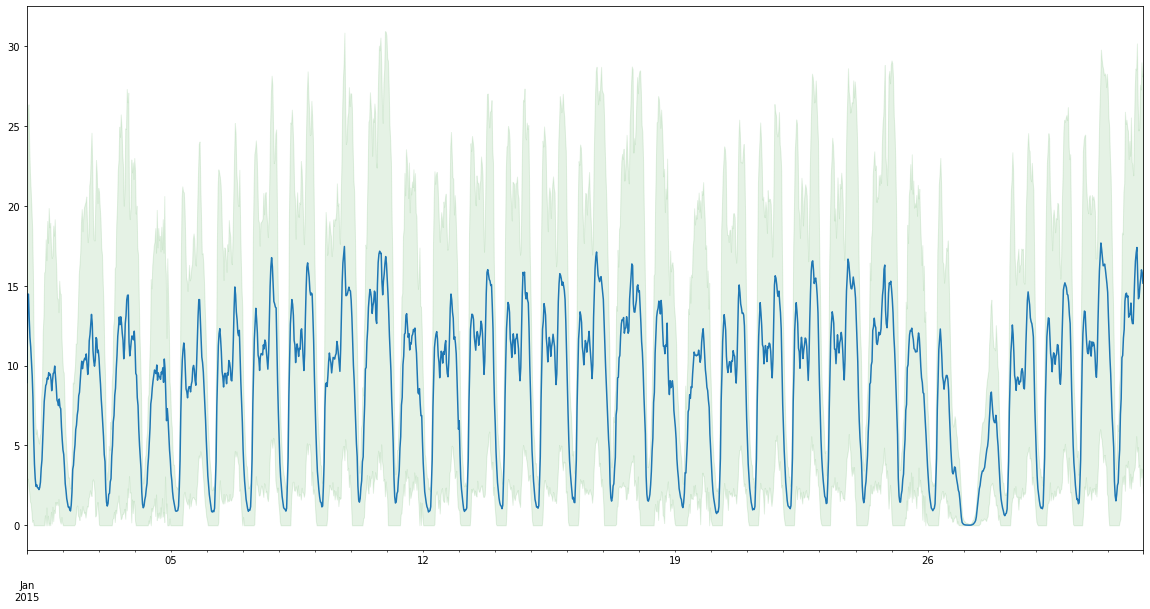
\includegraphics[width=\linewidth]{./img/taxi_30min_plot.png}
  \caption{Plot over the average timeseries in the taxi dataset with one standard deviation shown in green. Only positive values are shown as the dataset is non-negative.}
  \label{fig:taxi_30min_plot}
  \endminipage\hfill
\end{figure}

\begin{figure}[htb]
  \centering
  \minipage{0.4\textwidth}
  \begin{center}
    \begin{tabular}{||c | c | c | c | c |}
      \hline
      statistic   & mean & deviation & max  & min  \\
      \hline
      trend       & 0.02 & 0.02      & 0.16 & 0.0  \\
      \hline
      seasonality & 0.66 & 0.08      & 0.92 & 0.41 \\
      \hline
      \hline
    \end{tabular}
    \caption{Strength of trend and seasonality of the taxi dataset}
  \end{center}
  \endminipage\hfill
  \minipage{0.45\textwidth}
  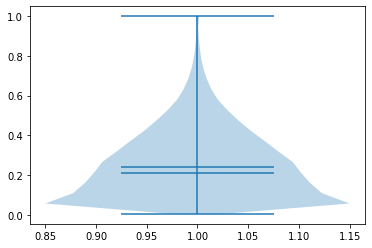
\includegraphics[width=\linewidth]{./img/taxi_30min_violin.png}
  \caption{Scaled violin plot of the taxi dataset.}
  \label{fig:taxi_30min_violin}
  \endminipage\hfill
\end{figure}

\clearpage
\subsection{M3 Monthly}

\begin{table}[htb]
  \begin{tabular}{||c | c c c c c c c ||}
    \hline
    Dataset & Mean    & Series & Items  & Shortest & Longest & Min      & Max      \\ [0.5ex]
    \hline\hline
    train   & 4928.47 & 1428   & 141858 & 48       & 126     & 80.00    & 86730.00 \\
    \hline
    test    & 4971.28 & 1428   & 167562 & 66       & 144     & -1200.00 & 86730.00 \\
    \hline
  \end{tabular}
  \caption{Statistics of the M3 Monthly dataset.}
\end{table}

\begin{figure}[htb]
  \centering
  \minipage{1.0\textwidth}
  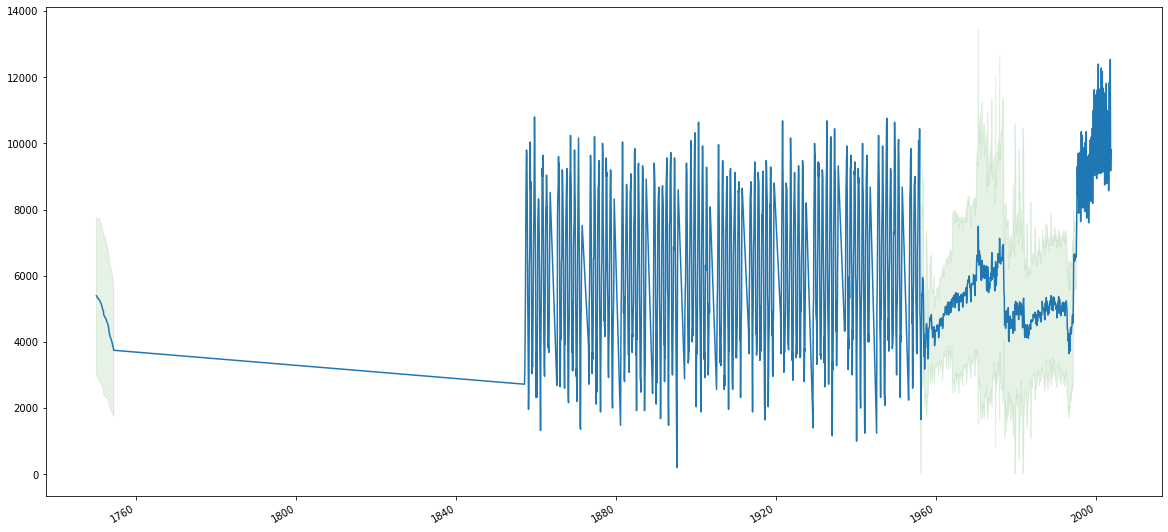
\includegraphics[width=\linewidth]{./img/m3_monthly_plot.png}
  \caption{Plot over the average timeseries in the m3 monthly dataset with one standard deviation shown in green. Only positive values are shown as the dataset is non-negative.}
  \label{fig:m3_monthly_plot}
  \endminipage\hfill
\end{figure}

\begin{figure}[htb]
  \centering
  \minipage{0.4\textwidth}
  \begin{center}
    \begin{tabular}{||c | c | c | c | c |}
      \hline
      statistic   & mean & deviation & max & min \\
      \hline
      trend       & 0.68 & 0.31      & 1.0 & 0.0 \\
      \hline
      seasonality & 0.35 & 0.29      & 1.0 & 0.0 \\
      \hline
      \hline
    \end{tabular}
    \caption{Strength of trend and seasonality of the m3 monthly dataset}
  \end{center}
  \endminipage\hfill
  \minipage{0.45\textwidth}
  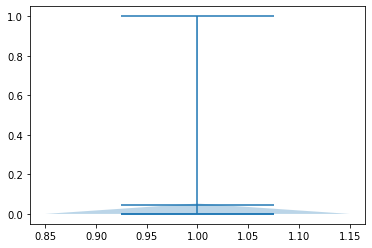
\includegraphics[width=\linewidth]{./img/m3_monthly_violin.png}
  \caption{Scaled violin plot of the m3 monthly dataset.}
  \label{fig:m3_monthly_violin}
  \endminipage\hfill
\end{figure}

\clearpage
\subsection{M3 Quarterly}
\begin{table}[htb]
  \begin{tabular}{||c | c c c c c c c ||}
    \hline
    Dataset & Mean    & Series & Items & Shortest & Longest & Min    & Max      \\ [0.5ex]
    \hline\hline
    train   & 4819.27 & 756    & 30956 & 16       & 64      & 126.00 & 20245.00 \\
    \hline
    test    & 4983.53 & 756    & 37004 & 24       & 72      & 121.00 & 20375.00 \\
    \hline
  \end{tabular}
  \caption{Statistics of the M3 Quarterly dataset.}
\end{table}
\begin{figure}[htb]
  \centering
  \minipage{1.0\textwidth}
  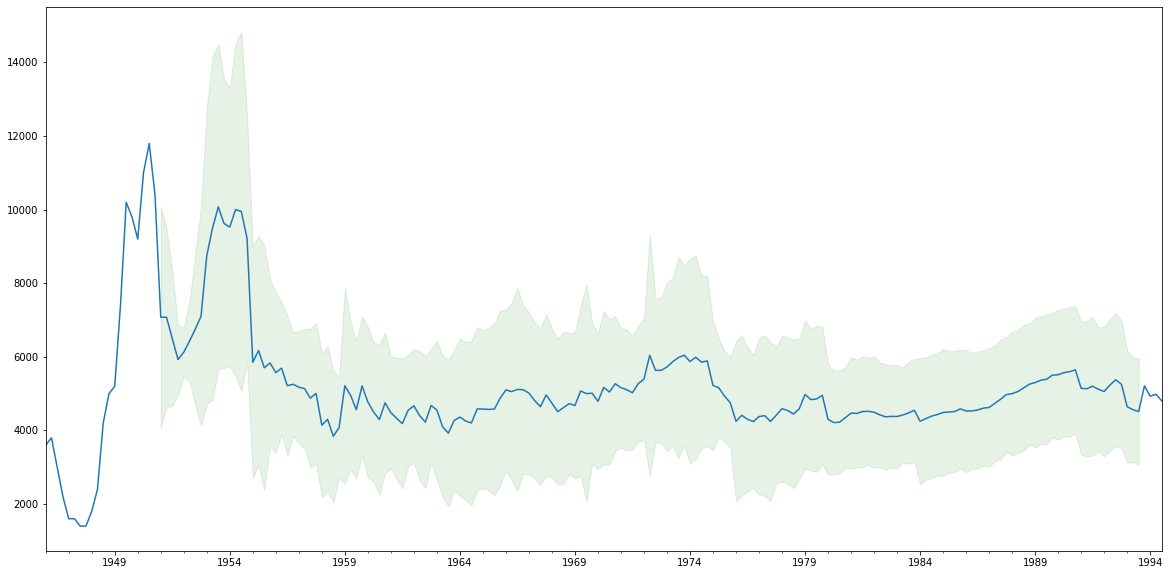
\includegraphics[width=\linewidth]{./img/m3_quarterly_plot.png}
  \caption{Plot over the average timeseries in the m3 quarterly dataset with one standard deviation shown in green. Only positive values are shown as the dataset is non-negative.}
  \label{fig:m3_quarterly_plot}
  \endminipage\hfill
\end{figure}

\begin{figure}[htb]
  \centering
  \minipage{0.4\textwidth}
  \begin{center}
    \begin{tabular}{||c | c | c | c | c |}
      \hline
      statistic   & mean & deviation & max & min \\
      \hline
      trend       & 0.88 & 0.19      & 1.0 & 0.0 \\
      \hline
      seasonality & 0.33 & 0.35      & 1.0 & 0.0 \\
      \hline
      \hline
    \end{tabular}
    \caption{Strength of trend and seasonality of the m3 quarterly dataset}
  \end{center}
  \endminipage\hfill
  \minipage{0.45\textwidth}
  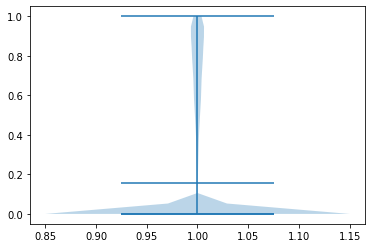
\includegraphics[width=\linewidth]{./img/m3_quarterly_violin.png}
  \caption{Scaled violin plot of the m3 quarterly dataset.}
  \label{fig:m3_quarterly_violin}
  \endminipage\hfill
\end{figure}

\clearpage
\subsection{M3 Yearly}
\begin{table}[htb]
  \begin{tabular}{||c | c c c c c c c ||}
    \hline
    Dataset & Mean    & Series & Items & Shortest & Longest & Min   & Max      \\ [0.5ex]
    \hline\hline
    train   & 4417.05 & 645    & 14449 & 14       & 41      & 30.00 & 39666.22 \\
    \hline
    test    & 4815.77 & 645    & 18319 & 20       & 47      & 30.00 & 45525.66 \\
    \hline
  \end{tabular}
  \caption{Statistics of the M3 Yearly dataset}
\end{table}
\begin{figure}[htb]
  \centering
  \minipage{1.0\textwidth}
  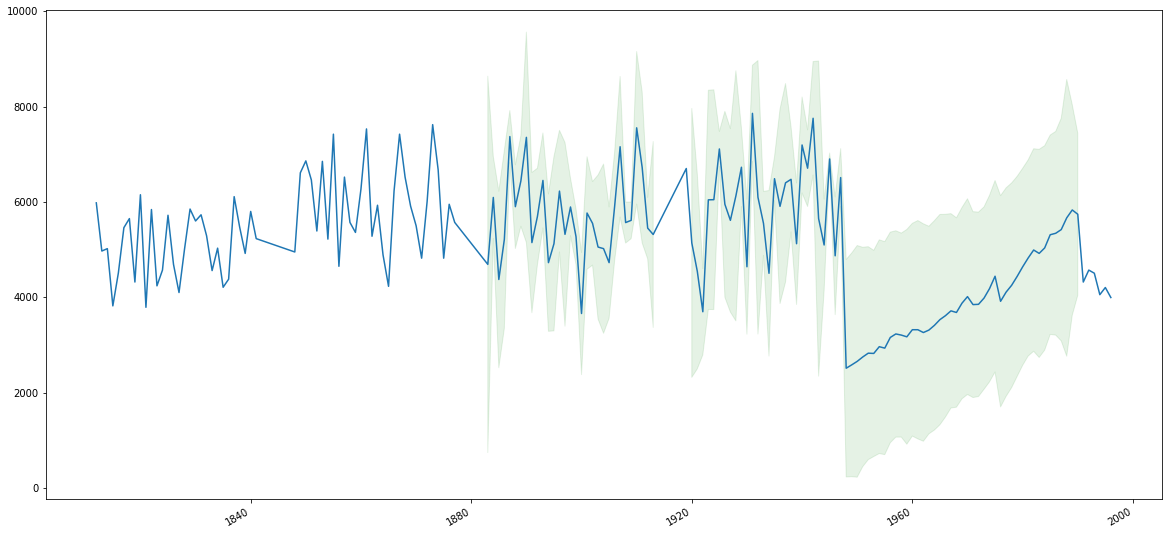
\includegraphics[width=\linewidth]{./img/m3_yearly_plot.png}
  \caption{Plot over the average timeseries in the m3 yearly dataset with one standard deviation shown in green. Only positive values are shown as the dataset is non-negative.}
  \label{fig:m3_yearly_plot}
  \endminipage\hfill
\end{figure}

\begin{figure}[htb]
  \centering
  \minipage{0.4\textwidth}
  \begin{center}
    \begin{tabular}{||c | c | c | c | c |}
      \hline
      statistic   & mean & deviation & max  & min \\
      \hline
      trend       & 0.89 & 0.17      & 1.0  & 0.0 \\
      \hline
      seasonality & 0.09 & 0.17      & 0.96 & 0.0 \\
      \hline
      \hline
    \end{tabular}
    \caption{Strength of trend and seasonality of the m3 yearly dataset}
  \end{center}
  \endminipage\hfill
  \minipage{0.45\textwidth}
  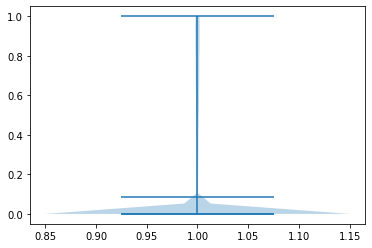
\includegraphics[width=\linewidth]{./img/m3_yearly_violin.png}
  \caption{Scaled violin plot of the m3 yearly dataset.}
  \label{fig:m3_yearly_violin}
  \endminipage\hfill
\end{figure}

\clearpage
\subsection{M3 Other}
\begin{table}[htb]
  \begin{tabular}{||c | c c c c c c c ||}
    \hline
    Dataset & Mean    & Series & Items & Shortest & Longest & Min   & Max      \\ [0.5ex]
    \hline\hline
    train   & 6152.18 & 174    & 11933 & 63       & 96      & 28.00 & 59472.00 \\
    \hline
    test    & 5999.87 & 174    & 13325 & 71       & 104     & 28.00 & 59472.00 \\
    \hline
  \end{tabular}
  \caption{Statistics of the M3 Other dataset}
\end{table}

\begin{figure}[htb]
  \centering
  \minipage{1.0\textwidth}
  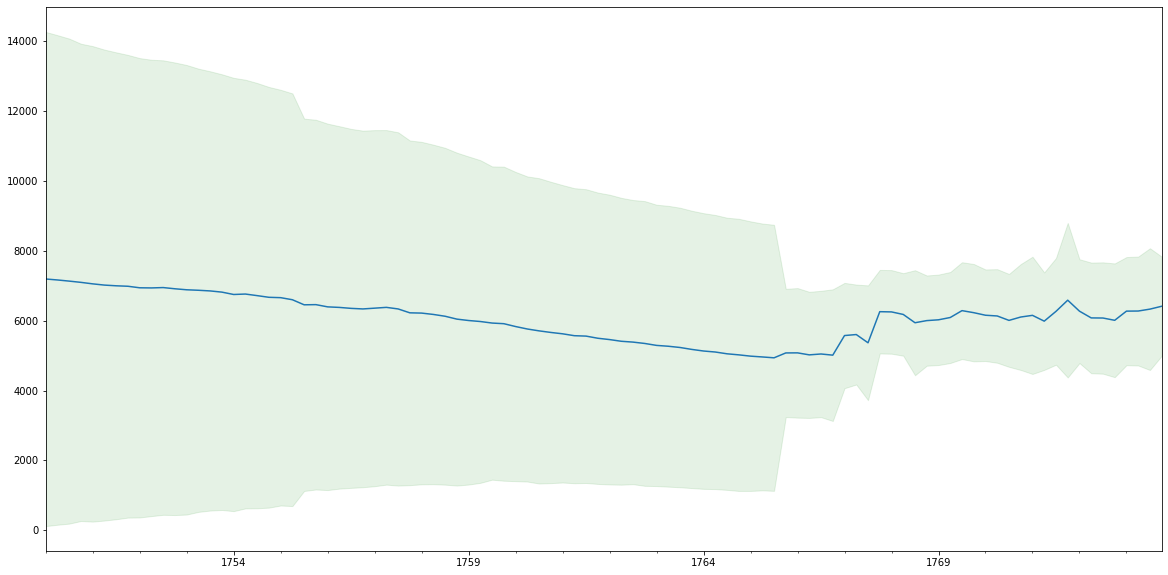
\includegraphics[width=\linewidth]{./img/m3_other_plot.png}
  \caption{Plot over the average timeseries in the m3 other dataset with one standard deviation shown in green. Only positive values are shown as the dataset is non-negative.}
  \label{fig:m3_other_plot}
  \endminipage\hfill
\end{figure}

\begin{figure}[htb]
  \centering
  \minipage{0.4\textwidth}
  \begin{center}
    \begin{tabular}{||c | c | c | c | c |}
      \hline
      statistic   & mean & deviation & max  & min  \\
      \hline
      trend       & 0.94 & 0.17      & 1.0  & 0.35 \\
      \hline
      seasonality & 0.07 & 0.08      & 0.44 & 0.0  \\
      \hline
      \hline
    \end{tabular}
    \caption{Strength of trend and seasonality of the m3 other dataset}
  \end{center}
  \endminipage\hfill
  \minipage{0.45\textwidth}
  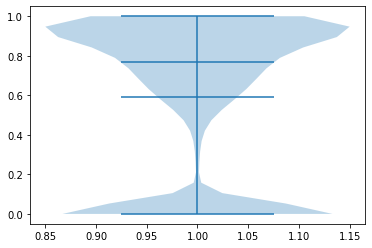
\includegraphics[width=\linewidth]{./img/m3_other_violin.png}
  \caption{Scaled violin plot of the m3 other dataset.}
  \label{fig:m3_other_violin}
  \endminipage\hfill
\end{figure}

\clearpage
\subsection{M4 Hourly}

\begin{table}[htb]
  \begin{tabular}{||c | c c c c c c c c ||}
    \hline
    Dataset & Mean    & Series & Items  & Shortest & Longest & Min   & Max       & Frequency \\ [0.5ex]
    \hline\hline
    train   & 6827.69 & 414    & 353500 & 700      & 960     & 10.00 & 703008.00 & H         \\
    \hline
    test    & 6859.56 & 414    & 373372 & 748      & 1008    & 10.00 & 703008.00 & H         \\
    \hline
  \end{tabular}
  \caption{Statistics of the M4 Hourly dataset}
\end{table}


\begin{figure}[htb]
  \centering
  \minipage{1.0\textwidth}
  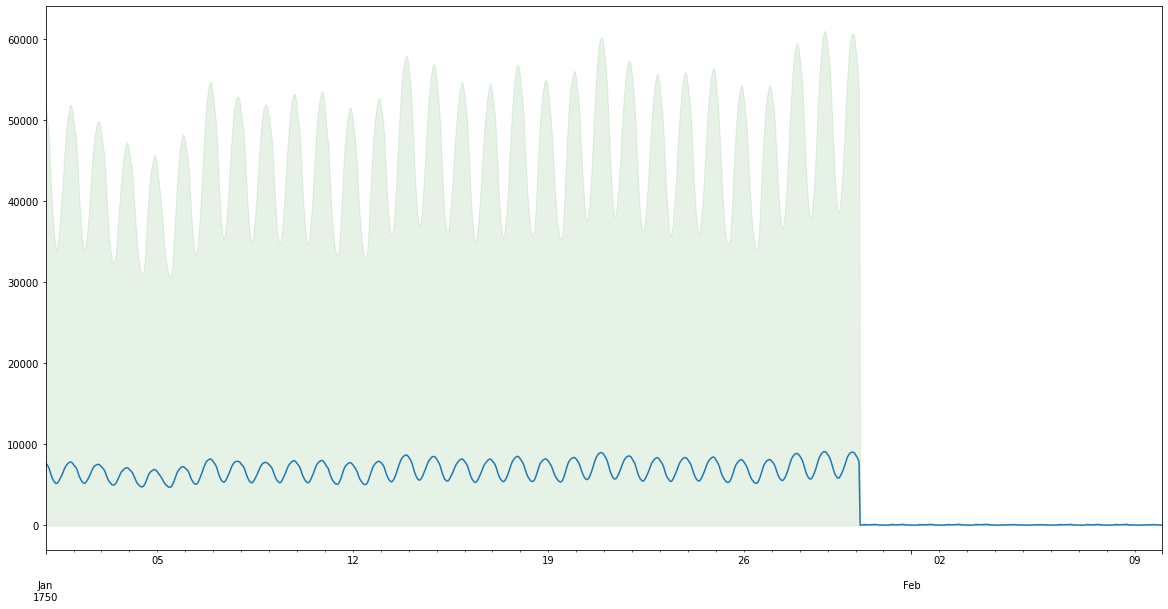
\includegraphics[width=\linewidth]{./img/m4_hourly_plot.png}
  \caption{Plot over the average timeseries in the m4 hourly dataset with one standard deviation shown in green. Only positive values are shown as the dataset is non-negative.}
  \label{fig:m4_hourly_plot}
  \endminipage\hfill
\end{figure}

\begin{figure}[htb]
  \centering
  \minipage{0.4\textwidth}
  \begin{center}
    \begin{tabular}{||c | c | c | c | c |}
      \hline
      statistic   & mean & deviation & max & min \\
      \hline
      trend       & 0.62 & 0.37      & 1.0 & 0.0 \\
      \hline
      seasonality & 0.88 & 0.16      & 1.0 & 0.0 \\
      \hline
      \hline
    \end{tabular}
    \caption{Strength of trend and seasonality of the m4 hourly dataset}
  \end{center}
  \endminipage\hfill
  \minipage{0.45\textwidth}
  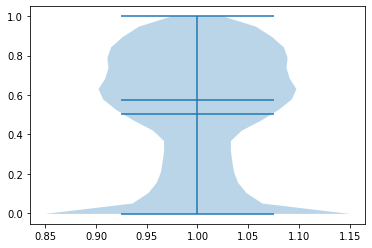
\includegraphics[width=\linewidth]{./img/m4_hourly_violin.png}
  \caption{Scaled violin plot of the m4 hourly dataset.}
  \label{fig:m4_hourly_violin}
  \endminipage\hfill
\end{figure}


\clearpage
\subsection{M4 Daily}
\begin{table}[htb]
  \begin{tabular}{||c | c c c c c c c c ||}
    \hline
    Dataset & Mean    & Series & Items    & Shortest & Longest & Min   & Max       & Frequency \\ [0.5ex]
    \hline\hline
    train   & 4951.40 & 4227   & 9964658  & 93       & 9919    & 15.00 & 352000.00 & D         \\
    \hline
    test    & 4960.15 & 4227   & 10023836 & 107      & 9933    & 15.00 & 352000.00 & D         \\
    \hline
  \end{tabular}
  \caption{Statistics of the M4 Daily dataset}
\end{table}

\begin{figure}[htb]
  \centering
  \minipage{1.0\textwidth}
  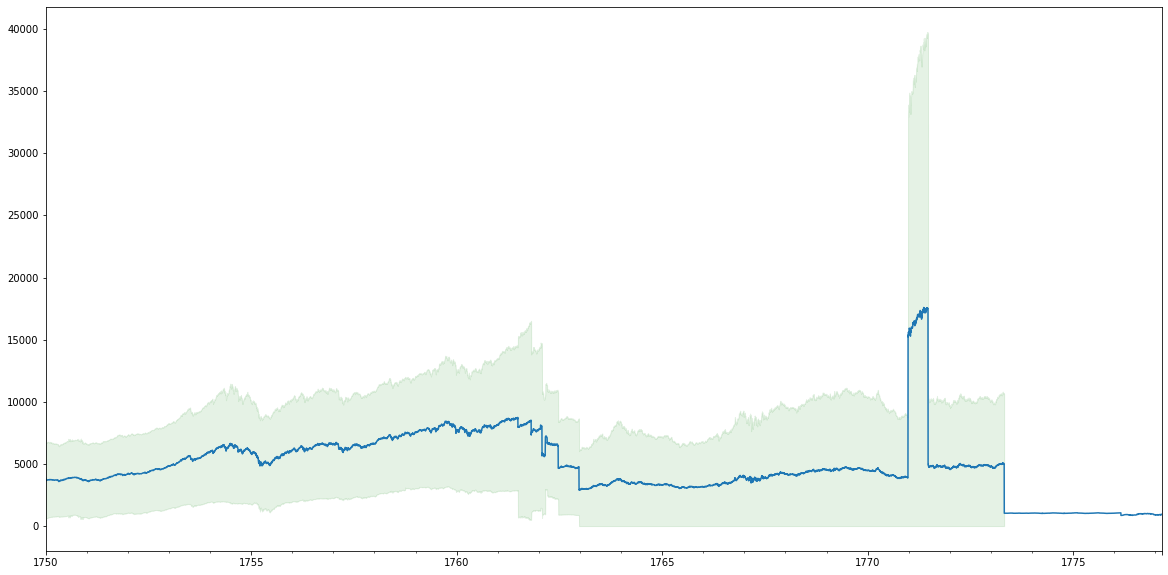
\includegraphics[width=\linewidth]{./img/m4_daily_plot.png}
  \caption{Plot over the average timeseries in the m4 daily dataset with one standard deviation shown in green. Only positive values are shown as the dataset is non-negative.}
  \label{fig:m4_daily_plot}
  \endminipage\hfill
\end{figure}

\begin{figure}[htb]
  \centering
  \minipage{0.4\textwidth}
  \begin{center}
    \begin{tabular}{||c | c | c | c | c |}
      \hline
      statistic   & mean & deviation & max & min \\
      \hline
      trend       & 0.98 & 0.05      & 1.0 & 0.0 \\
      \hline
      seasonality & 0.05 & 0.10      & 1.0 & 0.0 \\
      \hline
      \hline
    \end{tabular}
    \caption{Strength of trend and seasonality of the m4 daily dataset}
  \end{center}
  \endminipage\hfill
  \minipage{0.45\textwidth}
  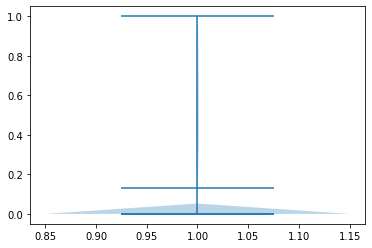
\includegraphics[width=\linewidth]{./img/m4_daily_violin.png}
  \caption{Scaled violin plot of the m4 daily dataset.}
  \label{fig:m4_daily_violin}
  \endminipage\hfill
\end{figure}

\clearpage
\subsection{M4 Weekly}
\begin{table}[htb]
  \begin{tabular}{||c | c c c c c c c c ||}
    \hline
    Dataset & Mean    & Series & Items  & Shortest & Longest & Min    & Max      & Frequency \\ [0.5ex]
    \hline\hline
    train   & 3738.52 & 359    & 366912 & 80       & 2597    & 104.69 & 51410.00 & W         \\
    \hline
    test    & 3755.97 & 359    & 371579 & 93       & 2610    & 104.69 & 51410.00 & W         \\
    \hline
  \end{tabular}
  \caption{Statistics of the M4 Weekly dataset}
\end{table}

\begin{figure}[htb]
  \centering
  \minipage{1.0\textwidth}
  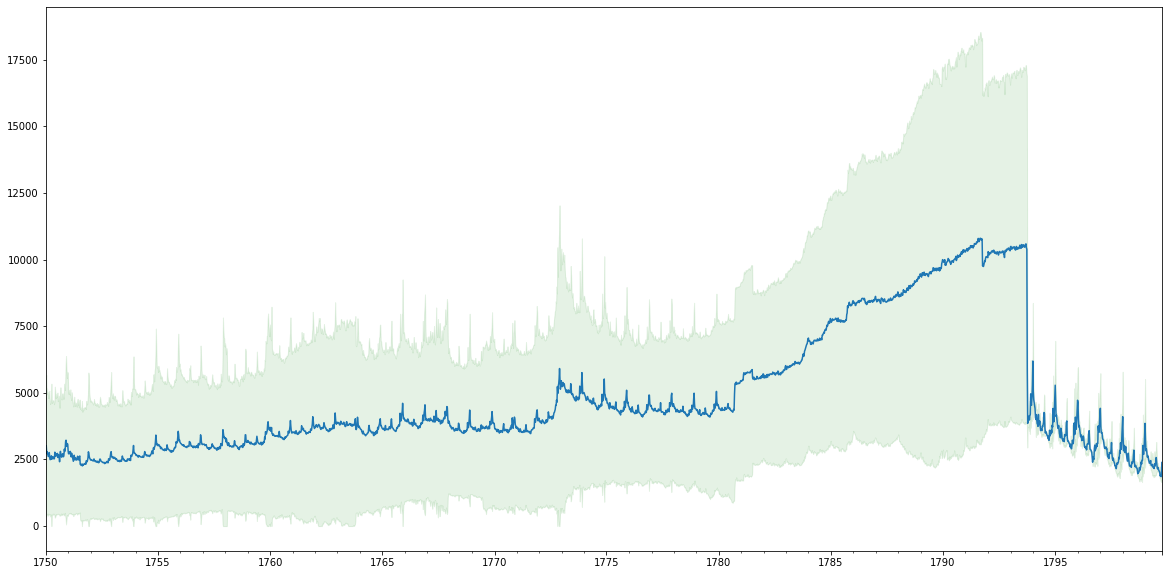
\includegraphics[width=\linewidth]{./img/m4_weekly_plot.png}
  \caption{Plot over the average timeseries in the m4 weekly dataset with one standard deviation shown in green. Only positive values are shown as the dataset is non-negative.}
  \label{fig:m4_weekly_plot}
  \endminipage\hfill
\end{figure}

\begin{figure}[htb]
  \centering
  \minipage{0.4\textwidth}
  \begin{center}
    \begin{tabular}{||c | c | c | c | c |}
      \hline
      statistic   & mean & deviation & max & min \\
      \hline
      trend       & 0.77 & 0.31      & 1.0 & 0.0 \\
      \hline
      seasonality & 0.34 & 0.35      & 1.0 & 0.0 \\
      \hline
      \hline
    \end{tabular}
    \caption{Strength of trend and seasonality of the m4 weekly dataset}
  \end{center}
  \endminipage\hfill
  \minipage{0.45\textwidth}
  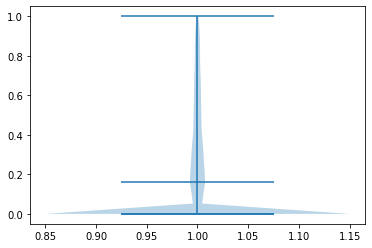
\includegraphics[width=\linewidth]{./img/m4_weekly_violin.png}
  \caption{Scaled violin plot of the m4 weekly dataset.}
  \label{fig:m4_weekly_violin}
  \endminipage\hfill
\end{figure}
\clearpage
\subsection{M4 Monthly}

\begin{table}[htb]
  \begin{tabular}{||c | c c c c c c c c ||}
    \hline
    Dataset & Mean    & Series & Items    & Shortest & Longest & Min   & Max       & Frequency \\ [0.5ex]
    \hline\hline
    train   & 4193.28 & 48000  & 10382411 & 42       & 2794    & 20.00 & 132731.31 & M         \\
    \hline
    test    & 4207.51 & 48000  & 11246411 & 60       & 2812    & 20.00 & 177950.00 & M         \\
    \hline
  \end{tabular}
  \caption{Statistics of the M4 Monthly dataset}
\end{table}


\begin{figure}[htb]
  \centering
  \minipage{1.0\textwidth}
  \includegraphics[width=\linewidth]{./img/m4_monthly_plot.png}
  \caption{Plot over the average timeseries in the m4 monthly dataset with one standard deviation shown in green. Only positive values are shown as the dataset is non-negative.}
  \label{fig:m4_monthly_plot}
  \endminipage\hfill
\end{figure}

\begin{figure}[htb]
  \centering
  \minipage{0.4\textwidth}
  \begin{center}
    \begin{tabular}{||c | c | c | c | c |}
      \hline
      statistic   & mean & deviation & max & min \\
      \hline
      trend       & 0.84 & 0.23      & 1.0 & 0.0 \\
      \hline
      seasonality & 0.32 & 0.30      & 1.0 & 0.0 \\
      \hline
      \hline
    \end{tabular}
    \caption{Strength of trend and seasonality of the m4 monthly dataset}
  \end{center}
  \endminipage\hfill
  \minipage{0.45\textwidth}
  \includegraphics[width=\linewidth]{./img/m4_monthly_violin.png}
  \caption{Scaled violin plot of the m4 monthly dataset.}
  \label{fig:m4_monthly_violin}
  \endminipage\hfill
\end{figure}

\clearpage
\subsection{M4 Quarterly}

\begin{table}[htb]
  \begin{tabular}{||c | c c c c c c c c ||}
    \hline
    Dataset & Mean    & Series & Items   & Shortest & Longest & Min   & Max      & Frequency \\ [0.5ex]
    \hline\hline
    train   & 4141.00 & 24000  & 2214108 & 16       & 866     & 19.50 & 82210.70 & 3M        \\
    \hline
    test    & 4287.13 & 24000  & 2406108 & 24       & 874     & 19.50 & 82210.70 & 3M        \\
    \hline
  \end{tabular}
  \caption{Statistics of the M4 Quarterly dataset}
\end{table}

\begin{figure}[htb]
  \centering
  \minipage{1.0\textwidth}
  \includegraphics[width=\linewidth]{./img/m4_quarterly_plot.png}
  \caption{Plot over the average timeseries in the m4 quarterly dataset with one standard deviation shown in green. Only positive values are shown as the dataset is non-negative.}
  \label{fig:m4_quarterly_plot}
  \endminipage\hfill
\end{figure}

\begin{figure}[htb]
  \centering
  \minipage{0.4\textwidth}
  \begin{center}
    \begin{tabular}{||c | c | c | c | c |}
      \hline
      statistic   & mean & deviation & max & min \\
      \hline
      trend       & 0.90 & 0.16      & 1.0 & 0.0 \\
      \hline
      seasonality & 0.20 & 0.27      & 1.0 & 0.0 \\
      \hline
      \hline
    \end{tabular}
    \caption{Strength of trend and seasonality of the m4 quarterly dataset}
  \end{center}
  \endminipage\hfill
  \minipage{0.45\textwidth}
  \includegraphics[width=\linewidth]{./img/m4_quarterly_violin.png}
  \caption{Scaled violin plot of the m4 quarterly dataset.}
  \label{fig:m4_quarterly_violin}
  \endminipage\hfill
\end{figure}

\clearpage
\subsection{M4 Yearly}
\begin{table}[htb]
  \begin{tabular}{||c | c c c c c c c c ||}
    \hline
    Dataset & Mean    & Series & Items  & Shortest & Longest & Min   & Max       & Frequency \\ [0.5ex]
    \hline\hline
    train   & 3630.52 & 23000  & 715065 & 13       & 300     & 22.10 & 115642.00 & 12M       \\
    \hline
    test    & 4076.24 & 23000  & 852909 & 19       & 300     & 22.00 & 158430.00 & 12M       \\
    \hline
  \end{tabular}
  \caption{Statistics of the M4 Yearly dataset}
\end{table}


\begin{figure}[htb]
  \centering
  \minipage{1.0\textwidth}
  \includegraphics[width=\linewidth]{./img/m4_yearly_plot.png}
  \caption{Plot over the average timeseries in the m4 yearly dataset with one standard deviation shown in green. Only positive values are shown as the dataset is non-negative.}
  \label{fig:m4_yearly_plot}
  \endminipage\hfill
\end{figure}

\begin{figure}[htb]
  \centering
  \minipage{0.4\textwidth}
  \begin{center}
    \begin{tabular}{||c | c | c | c | c |}
      \hline
      statistic   & mean & deviation & max  & min \\
      \hline
      trend       & 0.93 & 0.13      & 1.0  & 0.0 \\
      \hline
      seasonality & 0.09 & 0.16      & 0.98 & 0.0 \\
      \hline
      \hline
    \end{tabular}
    \caption{Strength of trend and seasonality of the m4 yearly dataset}
  \end{center}
  \endminipage\hfill
  \minipage{0.45\textwidth}
  \includegraphics[width=\linewidth]{./img/m4_yearly_violin.png}
  \caption{Scaled violin plot of the m4 yearly dataset.}
  \label{fig:m4_yearly_violin}
  \endminipage\hfill
\end{figure}


\clearpage
\subsection{M5}
\begin{table}[htb]
  \begin{tabular}{||c | c c c c c c c c ||}
    \hline
    Dataset & Mean & Series & Items    & Shortest & Longest & Min  & Max    & Frequency \\ [0.5ex]
    \hline\hline
    train   & 1.12 & 30490  & 57473650 & 1885     & 1885    & 0.00 & 763.00 & D         \\
    \hline
    test    & 1.13 & 30490  & 58327370 & 1913     & 1913    & 0.00 & 763.00 & D         \\
    \hline
  \end{tabular}
  \caption{Statistics of the M5 dataset}
\end{table}

\begin{figure}[htb]
  \centering
  \minipage{1.0\textwidth}
  \includegraphics[width=\linewidth]{./img/m5_plot.png}
  \caption{Plot over the average timeseries in the m5 dataset with one standard deviation shown in green. Only positive values are shown as the dataset is non-negative.}
  \label{fig:m5_plot}
  \endminipage\hfill
\end{figure}
\begin{figure}[htb]
  \centering
  \minipage{0.4\textwidth}
  \begin{center}
    \begin{tabular}{||c | c | c | c | c |}
      \hline
      statistic   & mean & deviation & max & min \\
      \hline
      trend       & 0.38 & 0.32      & 1.0 & 0.0 \\
      \hline
      seasonality & 0.28 & 0.33      & 1.0 & 0.0 \\
      \hline
      \hline
    \end{tabular}
    \caption{Strength of trend and seasonality of the m5 dataset}
  \end{center}
  \endminipage\hfill
  \minipage{0.45\textwidth}
  \includegraphics[width=\linewidth]{./img/m5_violin.png}
  \caption{Scaled violin plot of the m5 dataset.}
  \label{fig:m5_violin}
  \endminipage\hfill
\end{figure}
